\documentclass[12pt,english,ignorenonframetext,aspectratio=169,]{beamer}


%%%%%%%%%%%%%%%
%% Beamer theme
% choose one from http://deic.uab.es/~iblanes/beamer_gallery/
% or http://www.hartwork.org/beamer-theme-matrix/
% \usetheme{Warsaw}
\usetheme{CambridgeUS}

%%%%%%%%%%%%%%%%%%%%%%
%% Beamer color theme
%% default albatross beaver beetle crane dolphin dove fly lily
%% orchid rose seagull seahorse whale wolverine

%\usecolortheme{seahorse}  %% very lighty
\usecolortheme{dolphin}    %% nice blue
\usecolortheme{orchid}     %% dark red ?
\usecolortheme{whale}      %% black and blue as Warsaw

%%%%%%%%%%%%%%%%%%%%%%%%%%%%%%%%%%%%%%%%%%%%%%%%%%%%%%%%%%%%%%%%%%%%%%%%%%%%%%%%
%% Define your own colors
\definecolor{blackblue}{rgb}{19,19,59}  % rgb(48,48,150)

%%%%%%%%%%%%%%%%%%%%%%%%%%%%%%%%%%%%%%%%%%%%%%%%%%%%%%%%%%%%%%%%%%%%%%%%%%%%%%%%
%% Change the theme
%\setbeamercolor{alerted text}{fg=orange}
%\setbeamercolor{background canvas}{bg=white}
%\setbeamercolor{block body alerted}{bg=normal text.bg!90!black}
%\setbeamercolor{block body}{bg=normal text.bg!90!black}
%\setbeamercolor{block body example}{bg=normal text.bg!90!black}
%\setbeamercolor{block title alerted}{use={normal text,alerted text},fg=alerted text.fg!75!normal text.fg,bg=normal text.bg!75!black}
%\setbeamercolor{block title}{bg=blue}
%\setbeamercolor{block title example}{use={normal text,example text},fg=example text.fg!75!normal text.fg,bg=normal text.bg!75!black}
%\setbeamercolor{fine separation line}{}
\setbeamercolor{frametitle}{fg=black}
%\setbeamercolor{item projected}{fg=black}
%\setbeamercolor{normal text}{bg=black,fg=yellow}
%\setbeamercolor{palette sidebar primary}{use=normal text,fg=normal text.fg}
%\setbeamercolor{palette sidebar quaternary}{use=structure,fg=structure.fg}
%\setbeamercolor{palette sidebar secondary}{use=structure,fg=structure.fg}
%\setbeamercolor{palette sidebar tertiary}{use=normal text,fg=normal text.fg}
%\setbeamercolor{section in sidebar}{fg=brown}
%\setbeamercolor{section in sidebar shaded}{fg= grey}
\setbeamercolor{separation line}{}
%\setbeamercolor{sidebar}{bg=red}
%\setbeamercolor{sidebar}{parent=palette primary}
%\setbeamercolor{structure}{bg=black, fg=green}
%\setbeamercolor{subsection in sidebar}{fg=brown}
%\setbeamercolor{subsection in sidebar shaded}{fg= grey}
%\setbeamercolor{title}{fg=blackblue}
%\setbeamercolor{titlelike}{fg=blackblue}


%%%%%%%%%%%%%%%%%%%%%%%
%% Other beamer options
%\setbeamercovered{transparent}
% Permet de laisser en gris le texte qui n'est pas encore apparu (lorsqu'on utilise les commandes avec des <1,2> ou <4-9>.

%\setbeamercolor{normal text}{fg=black,bg=white}

%%%%%%%%%%%%%%%%%%%%%%%
%% Change Beamer fonts
% \usefonttheme{default}
% \usefonttheme[onlymath]{serif}
\usefonttheme{serif}

\setbeamerfont{title}{family=\rm}
\setbeamerfont{titlelike}{family=\rm}
\setbeamerfont{frametitle}{family=\rm}

%%%%%%%%%%%%%%%%%%%%%%%%%%%%%%%%%%%%%%%%%%%%%%%%%%%%%%%%%%%%%%%%%%%%%%%%%%%%%%%%
%% innertheme
%% rectangles circles inmargin rounded
% \useinnertheme{rounded}  % XXX My preference
\useinnertheme{circles}    % XXX

%%%%%%%%%%%%%%%%%%%%%%%%%%%%%%%%%%%%%%%%%%%%%%%%%%%%%%%%%%%%%%%%%%%%%%%%%%%%%%%%
%% outertheme
%% infolines miniframes shadow sidebar smoothbars smoothtree split tree
%\useoutertheme{infolines}

%% No navigation symbol.
\setbeamertemplate{navigation symbols}{}
\beamertemplatenavigationsymbolsempty

% XXX Add a background image to the slides
% \usepackage{tikz}
% \setbeamertemplate{background}{
\includegraphics[width=\paperwidth,height=\paperheight,keepaspectratio]{IETR.jpg}}
% \setbeamertemplate{background}{{\centering\begin{tikzpicture}\node[opacity=0.15]{
\includegraphics[width=0.98\paperwidth]{IETR_et_partenaires_IETR.png}};\end{tikzpicture}}}

% Other options
%\setbeamertemplate{footline}[page number]

\beamertemplateballitem
\setbeamertemplate{itemize item}[square]


\setbeamertemplate{caption}[numbered]
\setbeamertemplate{caption label separator}{: }
\setbeamercolor{caption name}{fg=normal text.fg}
\beamertemplatenavigationsymbolsempty
\usepackage{lmodern}
\usepackage{color}
  \newcommand{\urlb}[1]{\textcolor{blue}{\url{#1}}}
%% Color definition
\usepackage{xcolor}
%% WARNING attention when changing the colors, change both the {RGB}{r,g,b} and % rgb(r,g,b)
\definecolor{bleu}{RGB}{0,0,204}           % rgb(0,0,204)
\definecolor{deeppurple}{RGB}{102,0,204}   % rgb(102,0,204)
\definecolor{darkgreen}{RGB}{0,100,0}      % rgb(0,100,0)
\definecolor{yellowgreen}{RGB}{200,215,0}  % rgb(200,215,0)
\definecolor{bluegreen}{RGB}{0,185,140}    % rgb(0,185,140)
\definecolor{gold}{RGB}{255,180,0}         % rgb(255,180,0)
\definecolor{strongred}{RGB}{255,0,0}      % rgb(255,0,0)
\definecolor{normalred}{RGB}{204,0,0}      % rgb(204,0,0)
\definecolor{darkred}{RGB}{174,0,0}        % rgb(174,0,0)

\usepackage{amssymb,amsmath}
\usepackage{bbm,bm}  % bold maths symbols
\usepackage{ifxetex,ifluatex}
\usepackage{fixltx2e} % provides \textsubscript

% FIXME remove as soon as possible, it slows down compilation to import TikZ
%% TikZ
\usepackage{tikz}
\usetikzlibrary{snakes,arrows,shapes}
% https://tex.stackexchange.com/a/226974/
\tikzset{
  font={\fontsize{10pt}{10}\selectfont}
}
\usepackage{tikzsymbols}  % https://tex.stackexchange.com/a/227226/97964

\usepackage{macrosText}  % FIXME remove
\usepackage[linesnumbered,commentsnumbered,inoutnumbered,slide]{algorithm2e}


\ifnum 0\ifxetex 1\fi\ifluatex 1\fi=0 % if pdftex
  \usepackage[T1]{fontenc}
  \usepackage[utf8]{inputenc}
\else % if luatex or xelatex
  \ifxetex
    \usepackage{mathspec}
  \else
    \usepackage{fontspec}
  \fi
  \defaultfontfeatures{Ligatures=TeX,Scale=MatchLowercase}
\fi
% use upquote if available, for straight quotes in verbatim environments
\IfFileExists{upquote.sty}{\usepackage{upquote}}{}
% use microtype if available
\IfFileExists{microtype.sty}{%
\usepackage{microtype}
\UseMicrotypeSet[protrusion]{basicmath} % disable protrusion for tt fonts
}{}
\ifnum 0\ifxetex 1\fi\ifluatex 1\fi=0 % if pdftex
  \usepackage[shorthands=off,main=english]{babel}
\else
  \usepackage{polyglossia}
  \setmainlanguage[]{}
\fi
\newif\ifbibliography
\hypersetup{
            pdftitle={Multi-Player Bandits Revisited},
            pdfauthor={  Christophe Moy Émilie Kaufmann},
            pdfborder={0 0 0},
            breaklinks=true}
% \urlstyle{same}  % don't use monospace font for urls
% Code embedding.
\usepackage{palatino}              % Use the Palatino font % XXX remove if it is ugly ?

% Prevent slide breaks in the middle of a paragraph:
\widowpenalties 1 10000
\raggedbottom


\setlength{\parindent}{0pt}
\setlength{\parskip}{6pt plus 2pt minus 1pt}
\setlength{\emergencystretch}{3em}  % prevent overfull lines
\providecommand{\tightlist}{%
  \setlength{\itemsep}{0pt}\setlength{\parskip}{0pt}}
\setcounter{secnumdepth}{5}

% https://tex.stackexchange.com/a/2559/
\newcommand{\backupbegin}{
  \newcounter{framenumberappendix}
  \setcounter{framenumberappendix}{\value{framenumber}}
}
\newcommand{\backupend}{
  \addtocounter{framenumberappendix}{-\value{framenumber}}
  \addtocounter{framenumber}{\value{framenumberappendix}}
}

  \title{Multi-Player Bandits Revisited}
  \subtitle{Decentralized Multi-Player Multi-Arm Bandits}
    \author[Lilian Besson]{\textbf{Lilian Besson} \newline \emph{Advised by} \and Christophe Moy
\and Émilie Kaufmann}
        \institute[CentraleSupélec \& Inria]{PhD Student \newline Team SCEE, IETR, CentraleSupélec, Rennes
\newline \& Team SequeL, CRIStAL, Inria, Lille}
        \date[SequeL Seminar - 22/12/17]{SequeL Seminar - 22 December 2017}
  
% For \justifying command, see https://tex.stackexchange.com/a/148696/
\usepackage{ragged2e}
\addtobeamertemplate{frame begin}{}{\justifying}
\addtobeamertemplate{block begin}{}{\justifying}
\addtobeamertemplate{block alerted begin}{}{\justifying}
\addtobeamertemplate{block example begin}{}{\justifying}
\addtobeamertemplate{itemize body begin}{}{\justifying}
\addtobeamertemplate{itemize item}{}{\justifying}
\addtobeamertemplate{itemize subitem}{}{\justifying}
\addtobeamertemplate{itemize subsubitem}{}{\justifying}
\addtobeamertemplate{enumerate body begin}{}{\justifying}
\addtobeamertemplate{enumerate item}{}{\justifying}
\addtobeamertemplate{enumerate subitem}{}{\justifying}
\addtobeamertemplate{enumerate subsubitem}{}{\justifying}
\addtobeamertemplate{description body begin}{}{\justifying}
\addtobeamertemplate{description item}{}{\justifying}

\begin{document}
\justifying

\begin{frame}[plain]
\titlepage

% XXX manual inclusion of logos
\begin{center}

\includegraphics[height=0.13\textheight]{LogoIETR.png}

\includegraphics[height=0.13\textheight]{LogoCS.png}
\includegraphics[height=0.13\textheight]{LogoInria.jpg}
\end{center}

\end{frame}

\section*{\hfill{}CentraleSupélec Rennes \& Inria Lille\hfill{}}

\subsection*{\hfill{}Team {:} SCEE @ IETR \& SequeL @ CRIStAL\hfill{}}




\section{\hfill{}1. Introduction and motivation\hfill{}}

\subsection{\hfill{}1.a. Objective\hfill{}}

\end{frame}

\begin{frame}{Motivation}

We control some communicating devices, they want to access to a single
base station.

\begin{itemize}
\tightlist
\item
  Insert them in a \textbf{crowded wireless network}.
\item
  With a protocol \textbf{slotted in both time and frequency}.
\end{itemize}

\begin{block}{Goal}

\begin{itemize}
\tightlist
\item
  Maintain a \textbf{good Quality of Service}.
\item
  \textbf{With no centralized control} as it costs network overhead.
\end{itemize}

\end{block}

\begin{block}{How?}

\begin{itemize}
\tightlist
\item
  Devices can choose a different radio channel at each time \hook learn
  the best one with sequential algorithm!
\end{itemize}

\end{block}

\end{frame}



\subsection{\hfill{}1.b. Outline and references\hfill{}}

\end{frame}

\begin{frame}{Outline \uncover<2>{and reference}}

\vspace*{-15pt}

\begin{enumerate}
\def\labelenumi{\arabic{enumi}.}
\tightlist
\item
  \invisible{Introduction}
\item
  Our model: \(3\) different feedback levels
\item
  Decomposition and lower bound on regret
\item
  Quick reminder on single-player MAB algorithms
\item
  Two new multi-player decentralized algorithms
\item
  Upper bounds on regret for \MCTopM
\item
  Experimental results
\item
  An heuristic (\Selfish), and disappointing results
\item
  Conclusion
\end{enumerate}

\pause

\vfill{}

\begin{footnotesize}
This is based on our latest article:
\begin{itemize}
\item \emph{``Multi-Player Bandits Models Revisited''}, Besson \& Kaufmann. \hspace*{90pt}\texttt{\textcolor{blue}{\href{https://arXiv.org/abs/1711.02317}{arXiv:1711.02317}}}
\end{itemize}
\end{footnotesize}

\end{frame}



\section{\hfill{}2. Our model: $3$ different feedback level\hfill{}}

\subsection{\hfill{}2.a. Our model\hfill{}}

\end{frame}

\begin{frame}{Our model}

\begin{itemize}
\tightlist
\item
  \(K\) radio channels (\eg, 10) \hfill{} (\emph{known})
\item
  Discrete and synchronized time \(t\geq1\). Every time frame \(t\) is:
\end{itemize}

\begin{figure}[h!]
\centering
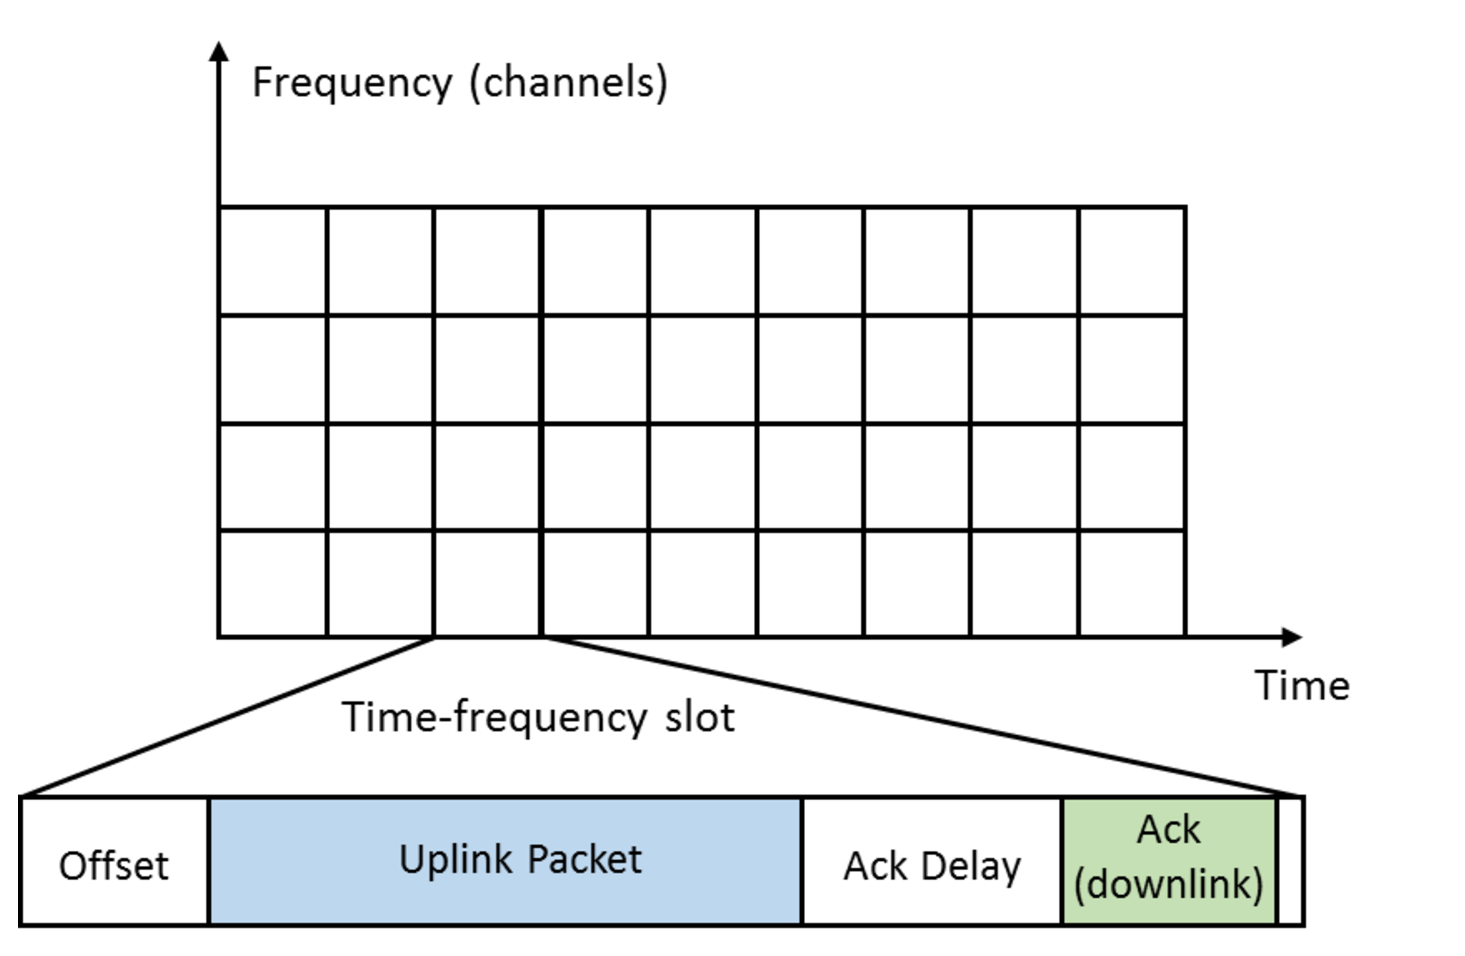
\includegraphics[height=0.27\textheight]{figures/protocol.eps}
\caption{\small{Protocol in time and frequency, with an \textcolor{darkgreen}{\emph{Acknowledgement}}.}}
\end{figure}

\begin{block}{Dynamic device \(=\) dynamic radio reconfiguration}

\begin{itemize}
\tightlist
\item
  It decides \textbf{each time} the channel it uses to send \textbf{each
  packet}.
\item
  It can implement a simple \textbf{decision algorithm}.
\end{itemize}

\end{block}

\end{frame}



\subsection{\hfill{}2.b. With or without sensing\hfill{}}

\end{frame}

\begin{frame}[fragile]{Our model}

\begin{block}{``Easy'' case}

\begin{itemize}
\tightlist
\item
  \(M \leq K\) devices \textbf{always communicate} and try to access the
  network, \emph{independently} without centralized supervision,
\item
  Background traffic is \iid.
\end{itemize}

\end{block}

\begin{block}{Two variants : with or without \emph{sensing}}

\begin{enumerate}
\def\labelenumi{\arabic{enumi}.}
\tightlist
\item
  \emph{With sensing}: Device first senses for presence of Primary Users
  (background traffic), then use \texttt{Ack} to detect collisions.

  \begin{quote}
  \small{Model the ``classical'' Opportunistic Spectrum Access problem.
  Not exactly suited for \emph{Internet of Things}, but can model ZigBee, and can be analyzed mathematically...}
  \end{quote}

  \pause
\item
  \emph{Without sensing}: same background traffic, but cannot sense, so
  only \texttt{Ack} is used.
  \small{More suited for ``IoT'' networks like LoRa or SigFox} (Harder to
  analyze mathematically.)
\end{enumerate}

\end{block}

\end{frame}



\subsection{\hfill{}2.c. Background traffic, and rewards\hfill{}}

\end{frame}

\begin{frame}{Background traffic, and rewards}

\begin{block}{\iid{} background traffic}

\begin{itemize}
\tightlist
\item
  \(K\) channels, modeled as Bernoulli (\(0/1\)) distributions of mean
  \(\mu_k\) \(=\) background traffic from \emph{Primary Users},
  bothering the dynamic devices,
\item
  \(M\) devices, each uses channel \(A^j(t) \in \{1,\dots,K\}\) at time
  \(t\).
\end{itemize}

\end{block}

\begin{block}{Rewards}

\[r^j(t) := Y_{A^j(t),t} \alert{\times} \mathbbm{1}(\overline{C^j(t)}) = \mathbbm{1}(\text{uplink \alert{\&} Ack})\]

\begin{itemize}
\tightlist
\item
  with sensing information
  \(\forall k, \;\; Y_{k,t} \overset{\text{iid}}{\sim} \mathrm{Bern}(\mu_k) \in \{0, 1\}\),
\item
  collision for device \(j\) :
  \(C^j(t) = \mathbbm{1}(\)\emph{alone on arm $A^j(t)$}\()\).
  \hook \alert{joint} binary reward \textbf{but not} from two Bernoulli!
\end{itemize}

\end{block}

\end{frame}



\subsection{\hfill{}2.d. Different feedback levels\hfill{}}

\end{frame}

\begin{frame}{3 feedback levels}

\only<1>{$$r^j(t) := \textcolor{red}{Y_{A^j(t),t}} \times \textcolor{blue}{\mathbbm{1}(\overline{C^j(t)})}$$}
\only<2>{$$r^j(t) := \textcolor{strongred}{Y_{A^j(t),t}} \times \textcolor{normalred}{\mathbbm{1}(\overline{C^j(t)})}$$}
\only<3>{$$r^j(t) := \textcolor{deeppurple}{Y_{A^j(t),t} \times \mathbbm{1}(\overline{C^j(t)})}$$}
\only<4>{$$\alert{r^j(t)} := Y_{A^j(t),t} \times \mathbbm{1}(\overline{C^j(t)})$$}

\begin{enumerate}
\def\labelenumi{\arabic{enumi}.}
\tightlist
\item
  ``Full \textcolor<1>{red}{feed}\textcolor<1>{blue}{back}'': observe
  both \textcolor<1>{red}{$Y_{A^j(t),t}$} \emph{and}
  \textcolor<1>{blue}{$C^j(t)$} separately, \hook Not realistic enough,
  we don't focus on it. \vspace*{10pt}\pause
\item
  \textcolor<2>{strongred}{``Sensing''}: first observe
  \(\textcolor<2>{strongred}{Y_{A^j(t),t}}\), \emph{then}
  \(\textcolor<2>{normalred}{C^j(t)}\) only if
  \(\textcolor<2>{strongred}{Y_{A^j(t),t}} \neq 0\), \hook Models
  licensed protocols (ex. ZigBee), our main focus. \vspace*{10pt}\pause
\item
  \textcolor<3>{deeppurple}{``No sensing''}: observe only the joint
  \(\textcolor<3>{deeppurple}{Y_{A^j(t),t} \times \mathbbm{1}(\overline{C^j(t)})}\),
  \hook Unlicensed protocols (ex. LoRaWAN), harder to analyze !
\end{enumerate}

\uncover<4>{\begin{quote}But all consider the same instantaneous \alert{reward $r^j(t)$}.\end{quote}}

\end{frame}



\subsection{\hfill{}2.e. Goal\hfill{}}

\end{frame}

\begin{frame}[fragile]{Goal}

\begin{block}{Problem}

\begin{itemize}
\tightlist
\item
  \emph{Goal} : \emph{minimize packet loss ratio} (\(=\) maximize nb of
  received \texttt{Ack}) in a \emph{finite-space discrete-time Decision
  Making Problem}.
\item
  \emph{Solution ?} \textbf{Multi-Armed Bandit algorithms},
  \textbf{decentralized} and used \textbf{independently} by each dynamic
  device.
\end{itemize}

\pause

\end{block}

\begin{block}{\emph{Decentralized} reinforcement learning optimization!}

\begin{itemize}
\tightlist
\item
  Max transmission rate \(\equiv\) \textbf{max cumulated rewards}
  \hspace*{0.25\textwidth}\(\max\limits_{\text{algorithm}\;A} \;\; \sum\limits_{t=1}^{T} \sum\limits_{j=1}^M r^j_{A(t)}\).
\item
  Each player wants to \textbf{maximize its cumulated reward},
\item
  With no central control, and no exchange of information,
\item
  Only possible if : each player converges to one of the \(M\) best
  arms, orthogonally (without collisions).
\end{itemize}

\end{block}

\end{frame}



\subsection{\hfill{}2.f. Centralized regret\hfill{}}

\end{frame}

\begin{frame}{Centralized regret}

\begin{block}{A measure of success}

\begin{itemize}
\tightlist
\item
  Not the network throughput or collision probability,
\item
  We study the \textbf{centralized} (expected) \textbf{regret}:
\end{itemize}

\begin{small}\vspace*{-20pt}
  $$R_T(\boldsymbol{\mu}, M, \rho)
  := \E_{\mu}\left[ \sum_{t=1}^T \sum_{j=1}^M \alert<1>{\mu_j^*} -  r^j(t)\right]
  \pause= \left(\sum_{k=1}^{M}\mu_k^*\right) T - \E_{\mu}\left[\sum_{t=1}^T\sum_{j=1}^M r^j(t)\right]$$
\end{small}

\vspace*{-10pt}

\pause

\end{block}

\begin{block}{Two directions of analysis}

\begin{itemize}
\tightlist
\item
  Clearly \(R_T = \mathcal{O}(T)\), but we want a sub-linear regret, as
  small as possible!\pause
\item
  \emph{How good a decentralized algorithm can be in this setting?}
  \hook{} \textbf{Lower Bound} on regret, for \textbf{any} algorithm !\pause
\item
  \emph{How good is my decentralized algorithm in this setting?}
  \hook{} \textbf{Upper Bound} on regret, for \textbf{one} algorithm !
\end{itemize}

\end{block}

\end{frame}



\section{\hfill{}3. Lower bound\hfill{}}

\end{frame}

\begin{frame}{Lower bound}

\begin{enumerate}
\def\labelenumi{\arabic{enumi}.}
\tightlist
\item
  Decomposition of regret in \(3\) terms,\vspace*{15pt}
\item
  Asymptotic lower bound of one term,\vspace*{15pt}
\item
  And for regret,\vspace*{15pt}
\item
  Sketch of proof,\vspace*{15pt}
\item
  Illustration.
\end{enumerate}

\end{frame}



\subsection{\hfill{}3.a. Lower bound on regret\hfill{}}

\end{frame}

\begin{frame}{Decomposition on regret}

\begin{block}{Decomposition}

For any algorithm, decentralized or not, we have \vspace*{-10pt}
\begin{footnotesize}\begin{align*}
R_T(\boldsymbol{\mu}, M, \rho) &= \alert<2>{\sum_{k \in \Mworst} (\mu_M^* -  \mu_k) \E_{\mu}[T_k(T)]} \\
&+ \alert<3>{\sum_{k \in \Mbest} (\mu_k -  \mu_M^*) \left(T - \E_{\mu}[T_k(T)]\right)} + \alert<4>{\sum_{k=1}^{K} \mu_k \E_{\mu}[\mathcal{C}_k(T)]}.
\end{align*}\end{footnotesize}
\vspace*{-10pt}

\end{block}

\begin{block}{Small regret can be attained if\ldots{}}

\pause

\begin{enumerate}
\def\labelenumi{\arabic{enumi}.}
\tightlist
\item
  Devices can quickly identify the bad arms \(\Mworst\), and not play
  them too much
  (\alert<2>{\emph{number of sub-optimal selections}}),\pause
\item
  Devices can quickly identify the best arms, and most surely play them
  (\alert<3>{\emph{number of optimal non-selections}}),\pause
\item
  Devices can use orthogonal channels
  (\alert<4>{\emph{number of collisions}}).
\end{enumerate}

\end{block}

\end{frame}

\begin{frame}{Asymptotic Lower Bound on regret I}

\begin{block}{\(3\) terms to lower bound\ldots{}}

\begin{itemize}
\tightlist
\item
  The first term for sub-optimal arms selections is lower bounded
  asymptotically,
  \[\forall\, \text{player}\, j, \text{bad arm}\,k,\; \mathop{\lim\inf}\limits_{T \to +\infty} \frac{\E_{\mu}[T_k^j(T)]}{\log T} \geq \frac{1}{\kl(\mu_k, \mu_M^*)},\]
  using technical information theory tools (Kullback-Leibler divergence,
  entropy),\pause
\item
  And we lower bound the rest (including collisions) by\ldots{} \(0\)
  \[T - \E_{\mu}[T_k(T)] \geq 0 \;\;\text{and}\;\;\; \E_{\mu}[\mathcal{C}_k(T)] \geq 0,\]
  \Sadey[1.4] we should be able to do better!
\end{itemize}

\end{block}

\end{frame}

\begin{frame}{Asymptotic Lower Bound on regret II}

\begin{block}{Theorem 1
\hfill{}\textcolor{gray}{[Besson \& Kaufmann, 2017]}}

\begin{itemize}
\tightlist
\item
  {\small For any uniformly efficient decentralized policy, and any
  non-degenerated problem \(\boldsymbol{\mu}\)}, \vspace*{-10pt}
  \[ \mathop{\lim\inf}\limits_{T \to +\infty} \frac{R_T(\boldsymbol{\mu}, M, \rho)}{\log(T)} \geq M \times \left( \sum_{k \in \Mworst} \frac{(\mu_M^* -  \mu_k)}{\kl(\mu_k, \mu_M^*)} \right) . \]
  \footnotetext{\tiny Where $\kl(x,y) := x \log(\frac{x}{y}) + (1 - x) \log(\frac{1-x}{1-y})$ is the \emph{binary} Kullback-Leibler divergence.}
\end{itemize}

\pause

\end{block}

\begin{block}{Remarks}

\begin{itemize}
\tightlist
\item
  The centralized \emph{multiple-play} lower bound is the same without
  the \(M\) multiplicative factor\ldots{}
  \citationright{Ref: [Anantharam et al, 1987]}
  \hook \alert{``price of non-coordination''} \(= M =\) nb of player?
\item
  Improved state-of-the-art lower bound, but still not perfect:
  collisions should also be controlled!
\end{itemize}

\end{block}

\end{frame}



\subsection{\hfill{}3.b. Illustration of the Lower Bound\hfill{}}

\end{frame}

\begin{frame}[plain]{Illustration of the Lower Bound on regret}

\begin{figure}[h!]
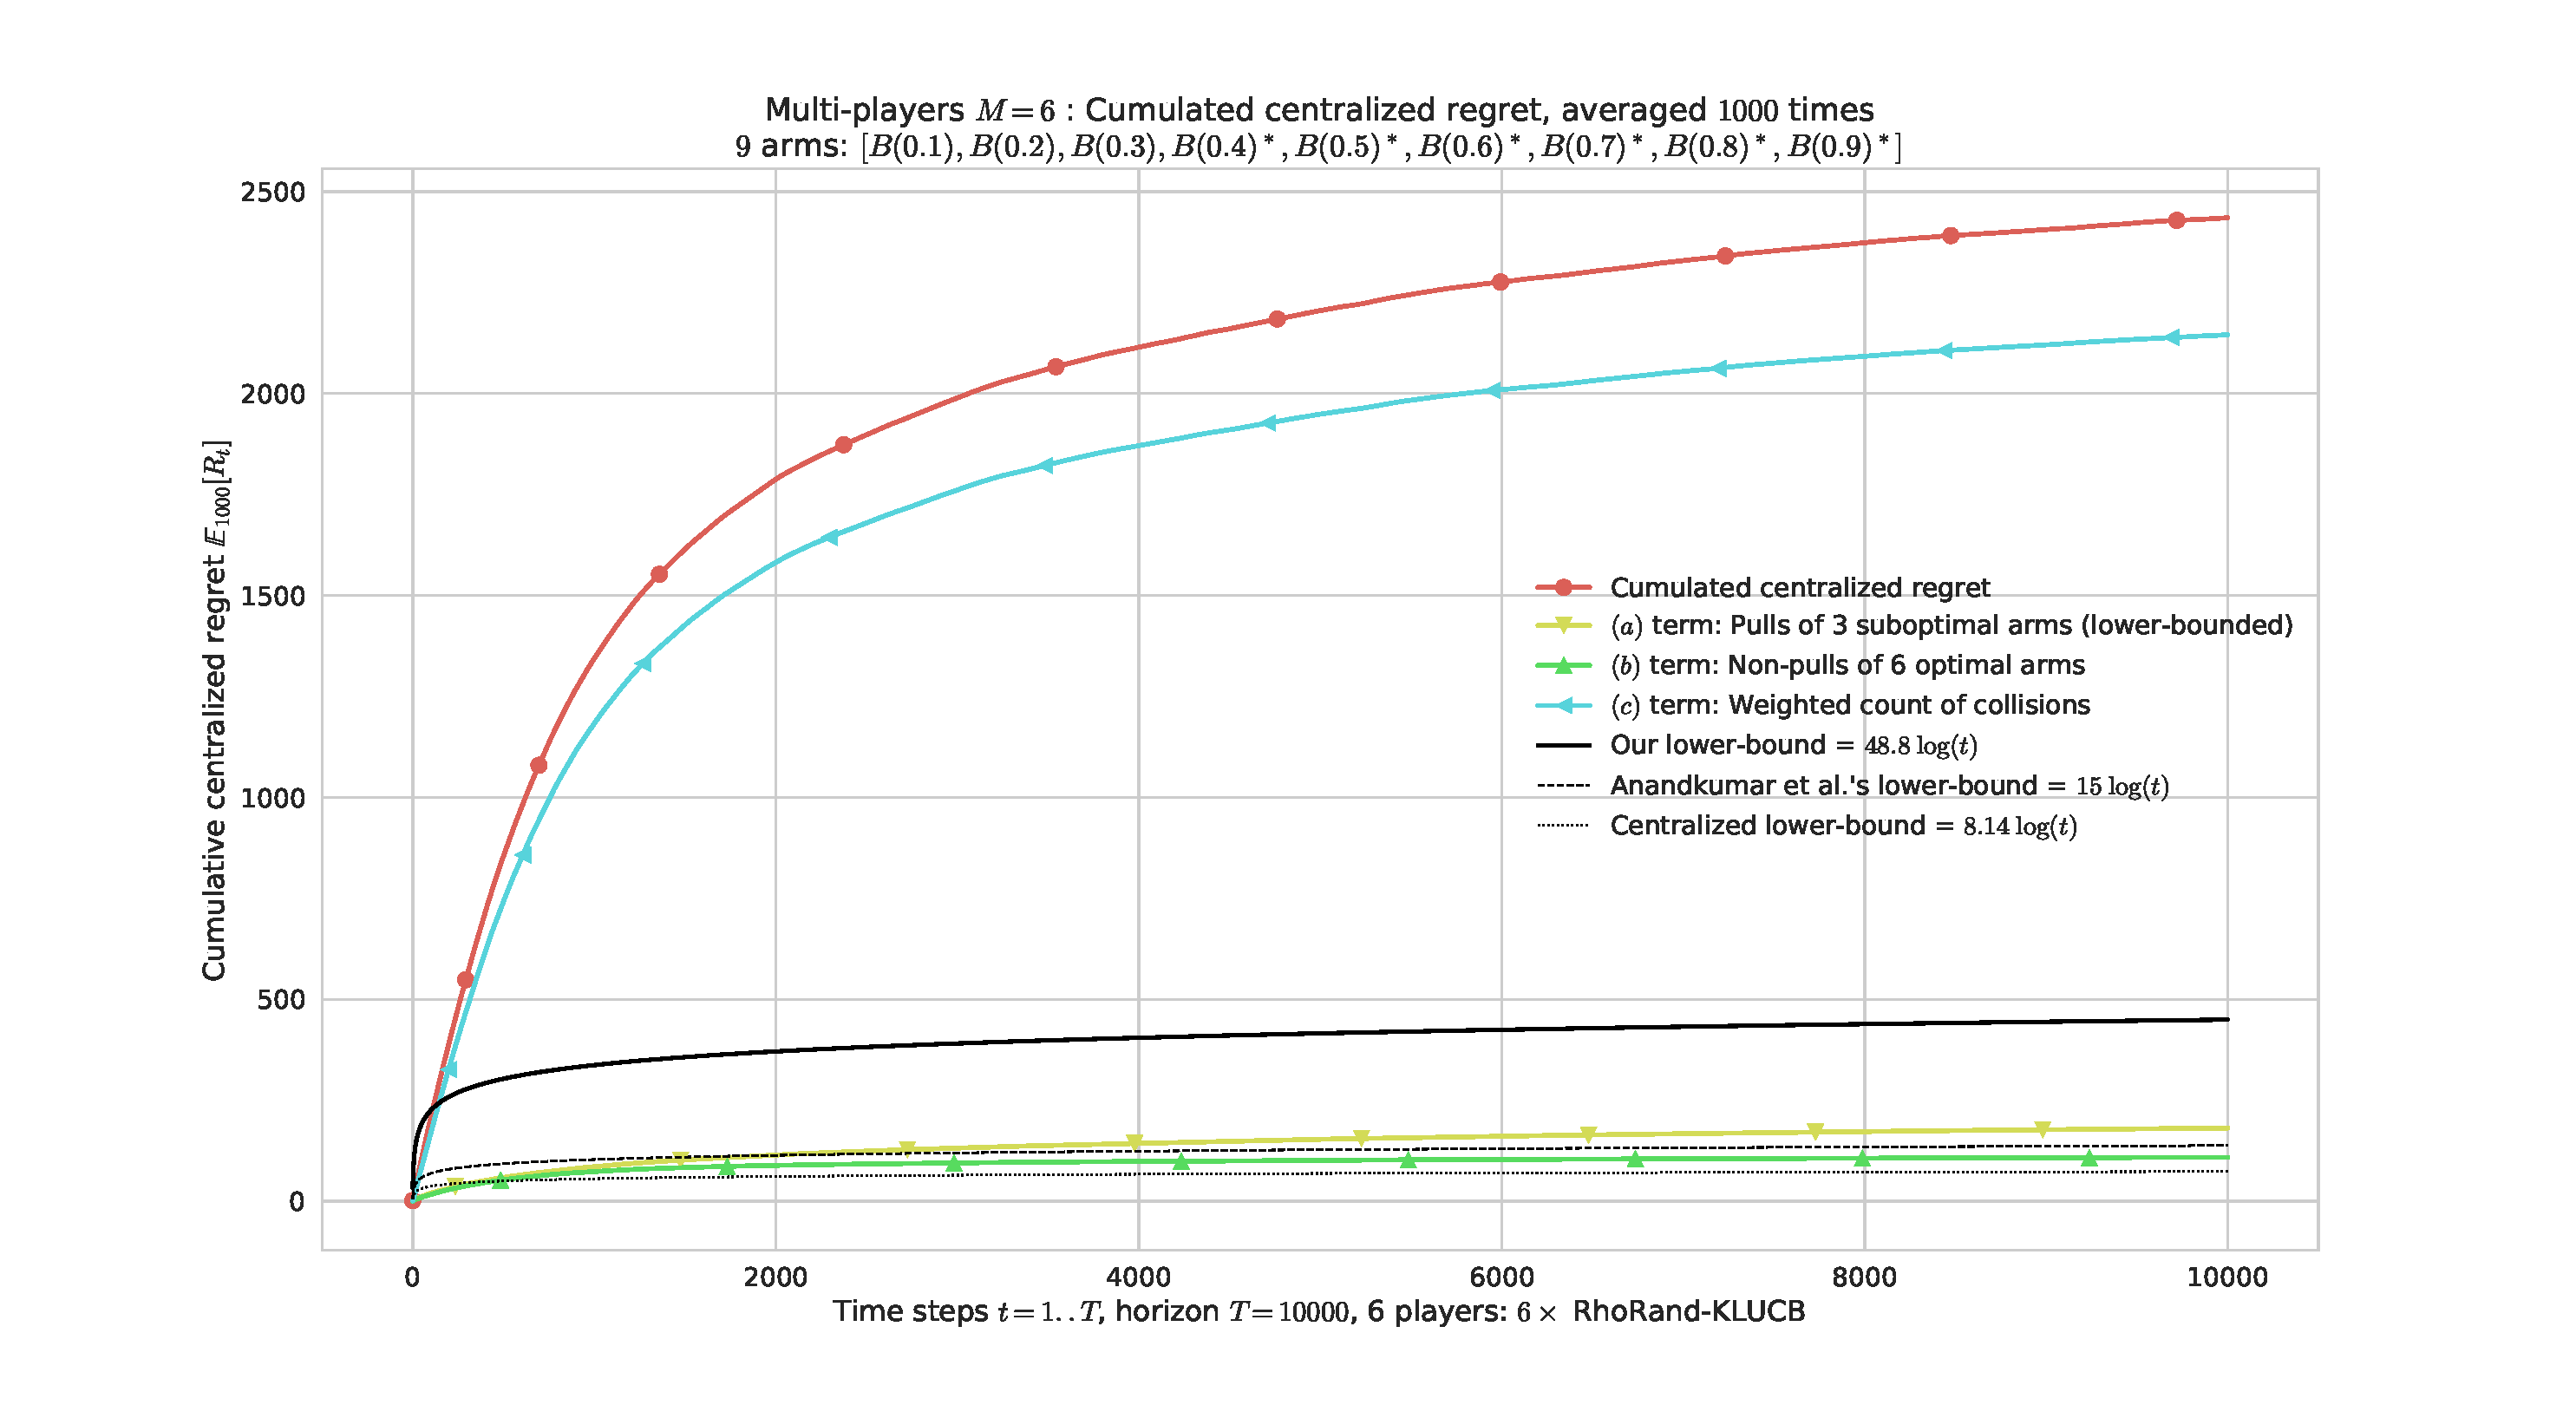
\includegraphics[height=0.80\textheight]{figures/main_RegretCentralized____env3-4_2092905764868974160.pdf}
\caption{\footnotesize{Any such lower bound is \alert{very asymptotic}, usually not satisfied for small horizons. We can see the importance of the collisions!}}
\end{figure}

\end{frame}



\subsection{\hfill{}3.c. Sketch of the proof\hfill{}}

\end{frame}

\begin{frame}{Sketch of the proof}

\begin{itemize}
\tightlist
\item
  Like for single-player bandit, focus on \(\E_{\mu}[T_k^j(T)]\)
  expected number of selections of any sub-optimal arm
  \(k\).\vspace*{10pt}
\item
  Same information-theoretic tools, using a ``change of law'' lemma.
  \citationright{[Garivier et al, 2016]}\vspace*{10pt}
\item
  It improved the state-of-the-art because of our decomposition, not
  because of new tools.
\end{itemize}

\begin{quote}
\strut

\hfill\(\hookrightarrow\) See our paper for details!
\end{quote}

\end{frame}



\section{\hfill{}4. Single-player MAB algorithms : \UCB, \klUCB\hfill{}}

\end{frame}

\begin{frame}{Single-player MAB algorithms}

\begin{enumerate}
\def\labelenumi{\arabic{enumi}.}
\tightlist
\item
  Index-based MAB deterministic policies,\vspace*{15pt}
\item
  Upper Confidence Bound algorithm : \UCB,\vspace*{15pt}
\item
  Kullback-Leibler UCB algorithm : \klUCB.
\end{enumerate}

\end{frame}



\subsection{\hfill{}4.a. Upper Confidence Bound algorithm : \UCB\hfill{}}

\end{frame}

\begin{frame}{Upper Confidence Bound algorithm (\(\mathrm{UCB}_1\))}

The device keep \(t\) number of sent packets, \(T_k(t)\) selections of
channel \(k\), \(X_k(t)\) successful transmissions in channel \(k\).

\begin{enumerate}
\def\labelenumi{\arabic{enumi}.}
\tightlist
\item
  For the first \(K\) steps (\(t=1,\dots,K\)), try each channel
  \emph{once}.
\item
  Then for the next steps \(t > K\) :

  \begin{itemize}
  \tightlist
  \item
    Compute the index
    \(g_k(t) := \underbrace{\frac{X_k(t)}{T_k(t)}}_{\text{Mean}\; \widehat{\mu_k}(t)} + \underbrace{\sqrt{\frac{\log(t)}{2 \; T_k(t)}},}_{\text{Upper Confidence Bound}}\)
  \item
    Choose channel \(A(t) = \mathop{\arg\max}\limits_{k} \; g_k(t)\),
  \item
    Update \(T_k(t+1)\) and \(X_k(t+1)\).
  \end{itemize}
\end{enumerate}

\citationbottomright{References: [Lai \& Robbins, 1985], [Auer et al, 2002], [Bubeck \& Cesa-Bianchi, 2012]}

\end{frame}



\subsection{\hfill{}4.b. Kullback-Leibler UCB algorithm : \klUCB\hfill{}}

\end{frame}

\begin{frame}{Kullback-Leibler UCB algorithm
(\(\mathrm{kl}\)-\(\mathrm{UCB}\))}

The device keep \(t\) number of sent packets, \(T_k(t)\) selections of
channel \(k\), \(X_k(t)\) successful transmissions in channel \(k\).

\begin{enumerate}
\def\labelenumi{\arabic{enumi}.}
\tightlist
\item
  For the first \(K\) steps (\(t=1,\dots,K\)), try each channel
  \emph{once}.
\item
  Then for the next steps \(t > K\) :

  \begin{itemize}
  \tightlist
  \item
    Compute the index
    \(g_k(t) := \sup\limits_{q \in [a, b]} \left\{ q : \mathrm{kl}\left(\frac{X_k(t)}{T_k(t)}, q\right) \leq \frac{\log(t)}{T_k(t)} \right\}\)
  \item
    Choose channel \(A(t) = \mathop{\arg\max}\limits_{k} \; g_k(t)\),
  \item
    Update \(T_k(t+1)\) and \(X_k(t+1)\).
  \end{itemize}
\end{enumerate}

\pause\alert<2>{\emph{Why bother?}} \klUCB{} is proved to be more
efficient than \UCB{}, and asymptotically optimal for single-player
stochastic bandit.

\citationbottomright{References: [Garivier \& Cappé, 2011], [Cappé \& Garivier \& Maillard \& Munos \& Stoltz, 2013]}

\end{frame}



\section{\hfill{}5. Multi-player decentralized algorithms\hfill{}}

\end{frame}

\begin{frame}{Multi-player decentralized algorithms}

\begin{enumerate}
\def\labelenumi{\arabic{enumi}.}
\tightlist
\item
  Common building blocks of previous algorithms,\vspace*{15pt}
\item
  First proposal: \RandTopM,\vspace*{15pt}
\item
  Second proposal: \MCTopM,\vspace*{15pt}
\item
  Algorithm and illustration.
\end{enumerate}

\end{frame}



\subsection{\hfill{}5.a. State-of-the-art MP algorithms\hfill{}}

\end{frame}

\begin{frame}{Algorithms for this easier model}

\begin{block}{Building blocks : separate the two aspects}

\begin{enumerate}
\def\labelenumi{\arabic{enumi}.}
\tightlist
\item
  \textbf{MAB policy} to learn the best arms (use sensing
  \(Y_{A^j(t),t}\)),
\item
  \textbf{Orthogonalization scheme} to avoid collisions (use
  \(C^j(t)\)).
\end{enumerate}

\pause

\end{block}

\begin{block}{Many different proposals for \emph{decentralized} learning
policies}

\begin{itemize}
\tightlist
\item
  Recent: \MEGA{} and \MusicalChair{},
  \citationright{[Avner \& Mannor, 2015], [Shamir et al, 2016]}
\item
  State-of-the-art: \rhoRand{} policy and variants.
  \citationright{[Anandkumar et al, 2011]}
\end{itemize}

\pause

\end{block}

\begin{block}{\textbf{Our proposals}:
\hfill{}\textcolor{gray}{[Besson \& Kaufmann, 2017]}}

\begin{itemize}
\tightlist
\item
  \emph{With sensing}: \RandTopM{} and \MCTopM{} are sort of mixes
  between \rhoRand{} and \MusicalChair, using UCB or more
  efficient index policies (\klUCB),
\item
  \emph{Without sensing}: \Selfish{} use a UCB index directly on the
  reward \(r^j(t)\).
\end{itemize}

\end{block}

\end{frame}



\subsection{\hfill{}5.b. \RandTopM{} algorithm\hfill{}}

\end{frame}

\begin{frame}{A first decentralized algorithm}

\centerline{\scalebox{0.80}{\begin{minipage}{1.25\textwidth}  %% https://tex.stackexchange.com/a/366403/
\begin{figure}[h!]
\centering
% Documentation at http://mirror.ctan.org/tex-archive/macros/latex/contrib/algorithm2e/doc/algorithm2e.pdf if needed
% Or https://en.wikibooks.org/wiki/LaTeX/Algorithms#Typesetting_using_the_algorithm2e_package
% \removelatexerror% Nullify \@latex@error % Cf. http://tex.stackexchange.com/a/82272/
\begin{algorithm}[H]
% XXX Input, data and output
% \KwIn{$K$ and policy $P^j$ for arms set $\{1,\dots,K\}$\;}
% \KwData{Data}
% \KwResult{Result}
% XXX Algorithm
Let $A^j(1) \sim \mathcal{U}(\{1,\dots,K\})$ and $C^j(1)=\mathrm{False}$ \\
\For{$t = 0, \dots, T - 1$}{
    %
    \eIf{$A^j(t) \notin \TopM(t)$ or $C^j(t)$}{
      $A^j(t+1) \sim \mathcal{U} \left(\TopM(t)\right)$
      \tcp*[f]{randomly switch}
      }{
        $A^j(t+1) = A^j(t)$
        \tcp*[f]{stays on the same arm}
      }
    Play arm $A^j(t+1)$, get new observations (sensing and collision), \\
    Compute the indices $g^j_k(t+1)$ and set $\TopM(t+1)$ for next step.
}
\caption{A first decentralized learning policy (for a fixed underlying index policy $g^j$). The set $\TopM(t)$ is the $M$ best arms according to indexes $g^j(t)$.}
\label{algo:firstAlgo}
\end{algorithm}
\end{figure}
\end{minipage}}}

\end{frame}

\begin{frame}{The \RandTopM{} algorithm}

\centerline{\scalebox{0.80}{\begin{minipage}{1.25\textwidth}  %% https://tex.stackexchange.com/a/366403/
\begin{figure}[h!]
\centering
% Documentation at http://mirror.ctan.org/tex-archive/macros/latex/contrib/algorithm2e/doc/algorithm2e.pdf if needed
% Or https://en.wikibooks.org/wiki/LaTeX/Algorithms#Typesetting_using_the_algorithm2e_package
% \removelatexerror% Nullify \@latex@error % Cf. http://tex.stackexchange.com/a/82272/
\begin{algorithm}[H]
% XXX Input, data and output
% \KwIn{$K$ and policy $P^j$ for arms set $\{1,\dots,K\}$\;}
% \KwData{Data}
% \KwResult{Result}
% XXX Algorithm
Let $A^j(1) \sim \mathcal{U}(\{1,\dots,K\})$ and $C^j(1)=\mathrm{False}$ \\
\For{$t = 0, \dots, T - 1$}{
    %
    \eIf{$A^j(t) \notin \TopM(t)$}{
      \eIf(\tcp*[f]{collision}){$C^j(t)$}{
        $A^j(t+1) \sim \mathcal{U} \left(\TopM(t)\right)$
        \tcp*[f]{randomly switch}
        }(\tcp*[f]{aim arm with smaller UCB at $t-1$}){
          $A^j(t+1) \sim \mathcal{U} \left(\TopM(t) \cap \left\{k : g_k^j(t-1) \leq g^j_{A^j(t)}(t-1)\right\}\right)$
        }
      }{
        $A^j(t+1) = A^j(t)$
        \tcp*[f]{stays on the same arm}
      }
    Play arm $A^j(t+1)$, get new observations (sensing and collision), \\
    Compute the indices $g^j_k(t+1)$ and set $\TopM(t+1)$ for next step.
}
\label{algo:RandTopM}
\end{algorithm}
\end{figure}
\end{minipage}}}

\end{frame}



\subsection{\hfill{}5.c. \MCTopM{} algorithm\hfill{}}

\end{frame}

\begin{frame}{The \MCTopM{} algorithm}

\begin{figure}[h!]
\scalebox{0.85}{\begin{minipage}{1.45\textwidth}  %% https://tex.stackexchange.com/a/366403/
\begin{tikzpicture}[>=latex',line join=bevel,scale=4.5]
    %
    \node (start) at (1.5,0.30) {$(0)$ Start $t=0$};
    \node (notfixed) at (1,0) [draw,rectangle,thick] {Not fixed, $\overline{s^j(t)}$};
    \node (fixed) at (0,0) [draw,rectangle,thick] {Fixed, $s^j(t)$};
    %
    \draw [black,->] (start) -> (notfixed.20);
    \draw [color=cyan,thick,->] (notfixed) to[bend right] node[midway,above,text width=5cm,text centered,black] {\small $(1)$ $\overline{C^j(t)}, A^j(t) \in \TopM(t)$} (fixed);
    \path [color=blue,thick,->] (notfixed) edge[loop right] node[right,text width=4cm,text badly centered,black] {\small $(2)$  $C^j(t), A^j(t) \in \TopM(t)$} (1);
    \path [color=red,thick,->] (notfixed) edge[loop below] node[below,text centered,black] {\small $(3)$  $A^j(t) \notin \TopM(t)$} (1);
    \path [color=darkgreen,thick,->] (fixed) edge[loop left] node[left,text width=2.9cm,text badly centered,black] {\small $(4)$ $A^j(t) \in \TopM(t)$} (fixed);
    \draw [color=red,thick,->] (fixed) to[bend right] node[midway,below,text centered,black] {\small $(5)$  $A^j(t) \notin \TopM(t)$} (notfixed);
    %
\end{tikzpicture}
\end{minipage}}
\caption{\small Player $j$ using $\mathrm{MCTopM}$, represented as ``state machine'' with $5$ transitions.
Taking one of the five transitions means playing one round of Algorithm \MCTopM, to decide $A^j(t+1)$ using information of previous steps.}
\label{fig:StateMachineAlgorithm_MCTopM}
\end{figure}

\end{frame}

\begin{frame}[plain]{The \MCTopM{} algorithm}

\centerline{\scalebox{0.78}{\begin{minipage}{1.25\textwidth}  %% https://tex.stackexchange.com/a/366403/
\begin{figure}[h!]
\centering
% Documentation at http://mirror.ctan.org/tex-archive/macros/latex/contrib/algorithm2e/doc/algorithm2e.pdf if needed
% Or https://en.wikibooks.org/wiki/LaTeX/Algorithms#Typesetting_using_the_algorithm2e_package
% \removelatexerror% Nullify \@latex@error % Cf. http://tex.stackexchange.com/a/82272/
\begin{algorithm}[H]
% XXX Input, data and output
% \KwIn{$K$ and policy $P^j$ for arms set $\{1,\dots,K\}$\;}
% \KwData{Data}
% \KwResult{Result}
% XXX Algorithm
Let $A^j(1) \sim \mathcal{U}(\{1,\dots,K\})$ and $C^j(1)=\mathrm{False}$ and $s^j(1)=\mathrm{False}$ \\
\For{$t = 0, \dots, T-1$}{
      \uIf(\tcp*[f]{\textcolor{red}{transition $(3)$ or $(5)$}}){
        $A^j(t) \notin \TopM(t)$}
      {
        $A^j(t+1) \sim \mathcal{U} \left(\TopM(t) \cap \left\{k : g_k^j(t-1) \leq g^j_{A^j(t)}(t-1)\right\}\right)$
        \tcp*[f]{not empty} \\
        $s^j(t+1) = \mathrm{False}$
        \tcp*[f]{aim at an arm with smaller UCB at $t-1$}
      }
      \uElseIf(\tcp*[f]{collision and not fixed}){
          $C^j(t)$ \emph{and} $\overline{s^j(t)}$}
        {
          $A^j(t+1) \sim \mathcal{U} \left(\TopM(t)\right)$
          \tcp*[f]{\textcolor{blue}{transition $(2)$}} \\
          $s^j(t+1) = \mathrm{False}$
      }
      \Else(\tcp*[f]{transition \textcolor{cyan}{$(1)$} or \textcolor{darkgreen}{$(4)$}}){
        $A^j(t+1) = A^j(t)$ \tcp*[f]{stay on the previous arm} \\
        $s^j(t+1) = \mathrm{True}$ \tcp*[f]{become or stay fixed on a ``chair''}
      }
    Play arm $A^j(t+1)$, get new observations (sensing and collision), \\
    Compute the indices $g^j_k(t+1)$ and set $\TopM(t+1)$ for next step.
}
\label{algo:MCTopM}
\end{algorithm}
\end{figure}
\end{minipage}}}

\end{frame}



\section{\hfill{}6. Regret upper bound\hfill{}}

\end{frame}

\begin{frame}{Regret upper bound}

\begin{enumerate}
\def\labelenumi{\arabic{enumi}.}
\tightlist
\item
  Theorem,\vspace*{15pt}
\item
  Remarks,\vspace*{15pt}
\item
  Idea of the proof.
\end{enumerate}

\end{frame}



\subsection{\hfill{}6.a. Theorem for \MCTopM{} with \klUCB\hfill{}}

\end{frame}

\begin{frame}{Regret upper bound for \MCTopM{}}

\begin{block}{Theorem 2
\hfill{}\textcolor{gray}{[Besson \& Kaufmann, 2017]}}

\begin{itemize}
\tightlist
\item
  If all \(M\) players use \MCTopM{} with \klUCB, then for any
  non-degenerated problem \(\boldsymbol{\mu}\), there exists a problem
  dependent constant \(G_{M,\boldsymbol{\mu}}\) , such that the regret
  satisfies: \[
  R_T(\boldsymbol{\mu}, M, \rho) \leq G_{M,\boldsymbol{\mu}} \log(T) + \smallO{\log T}.
    \]
\end{itemize}

\pause

\end{block}

\begin{block}{How?}

\begin{itemize}
\tightlist
\item
  Decomposition of regret controlled with two terms,
\item
  Control both terms, both are logarithmic:

  \begin{itemize}
  \tightlist
  \item
    Suboptimal selections with the ``classical analysis'' on \klUCB{}
    indexes
  \item
    Collisions are harder to control\ldots{}
  \end{itemize}
\end{itemize}

\end{block}

\end{frame}

\begin{frame}{Regret upper bound for \MCTopM{}}

\begin{block}{Remarks}

\begin{itemize}
\tightlist
\item
  Hard to prove, we had to carefully design the \MCTopM{} algorithm to
  conclude the proof,\pause
\item
  The constant \(G_{M,\boldsymbol{\mu}}\) scales as \(M^3\), way better
  than \rhoRand's constant scaling as \(M{2M-1 \choose M}\),\pause
\item
  We also \emph{minimize the number of channel switching}: interesting
  as changing arm costs energy in radio systems,\pause
\item
  For the suboptimal selections, we \emph{match our lower bound} !\pause
\item
  Not yet possible to know what is the best possible control of
  collisions\ldots{}
\end{itemize}

\end{block}

\end{frame}



\subsection{\hfill{}6.b. Sketch of the proof\hfill{}}

\end{frame}

\begin{frame}{Sketch of the proof}

\begin{enumerate}
\def\labelenumi{\arabic{enumi}.}
\tightlist
\item
  Bound the expected number of collisions by \(M\) times the number of
  collisions for non-sitted players,\pause
\item
  Bound the expected number of
  \textcolor<2>{red}{transitions of type $(3)$ and $(5)$}, by
  \(\bigO{\log T}\) using the \klUCB{} indexes and the forced choice of
  the algorithm:
  \(g_k^j(t-1) \leq g^j_{k'}(t-1), \;\;\text{and}\;\; g_k^j(t) > g^j_{k'}(t)\)
  when switching from \(k'\) to \(k\),\pause
\item
  Bound the expected length of a sequence in the non-sitted state by a
  constant,\pause
\item
  So most of the times (\(\bigO{T - \log T}\)), players are sitted, and
  no collision happens when they are all sitted!
\end{enumerate}

\begin{quote}
\strut

\hfill\(\hookrightarrow\) See our paper for details!
\end{quote}

\end{frame}



\section{\hfill{}7. Experimental results\hfill{}}

\end{frame}

\begin{frame}{Experimental results}

\begin{quote}
Experiments on Bernoulli problems \(\boldsymbol{\mu}\in[0,1]^K\).
\end{quote}

\begin{enumerate}
\def\labelenumi{\arabic{enumi}.}
\tightlist
\item
  Illustration of regret for a single problem and
  \(M = K\),\vspace*{15pt}
\item
  Regret for uniformly sampled problems and \(M < K\),\vspace*{15pt}
\item
  Logarithmic number of collisions,\vspace*{15pt}
\item
  Logarithmic number of arm switches,\vspace*{15pt}
\item
  Fairness?
\end{enumerate}

\end{frame}



\subsection{\hfill{}7.a. Illustration of regret\hfill{}}

\end{frame}

\begin{frame}[plain]{Constant regret if \(M=K\)}

\begin{figure}[h!]
\centering
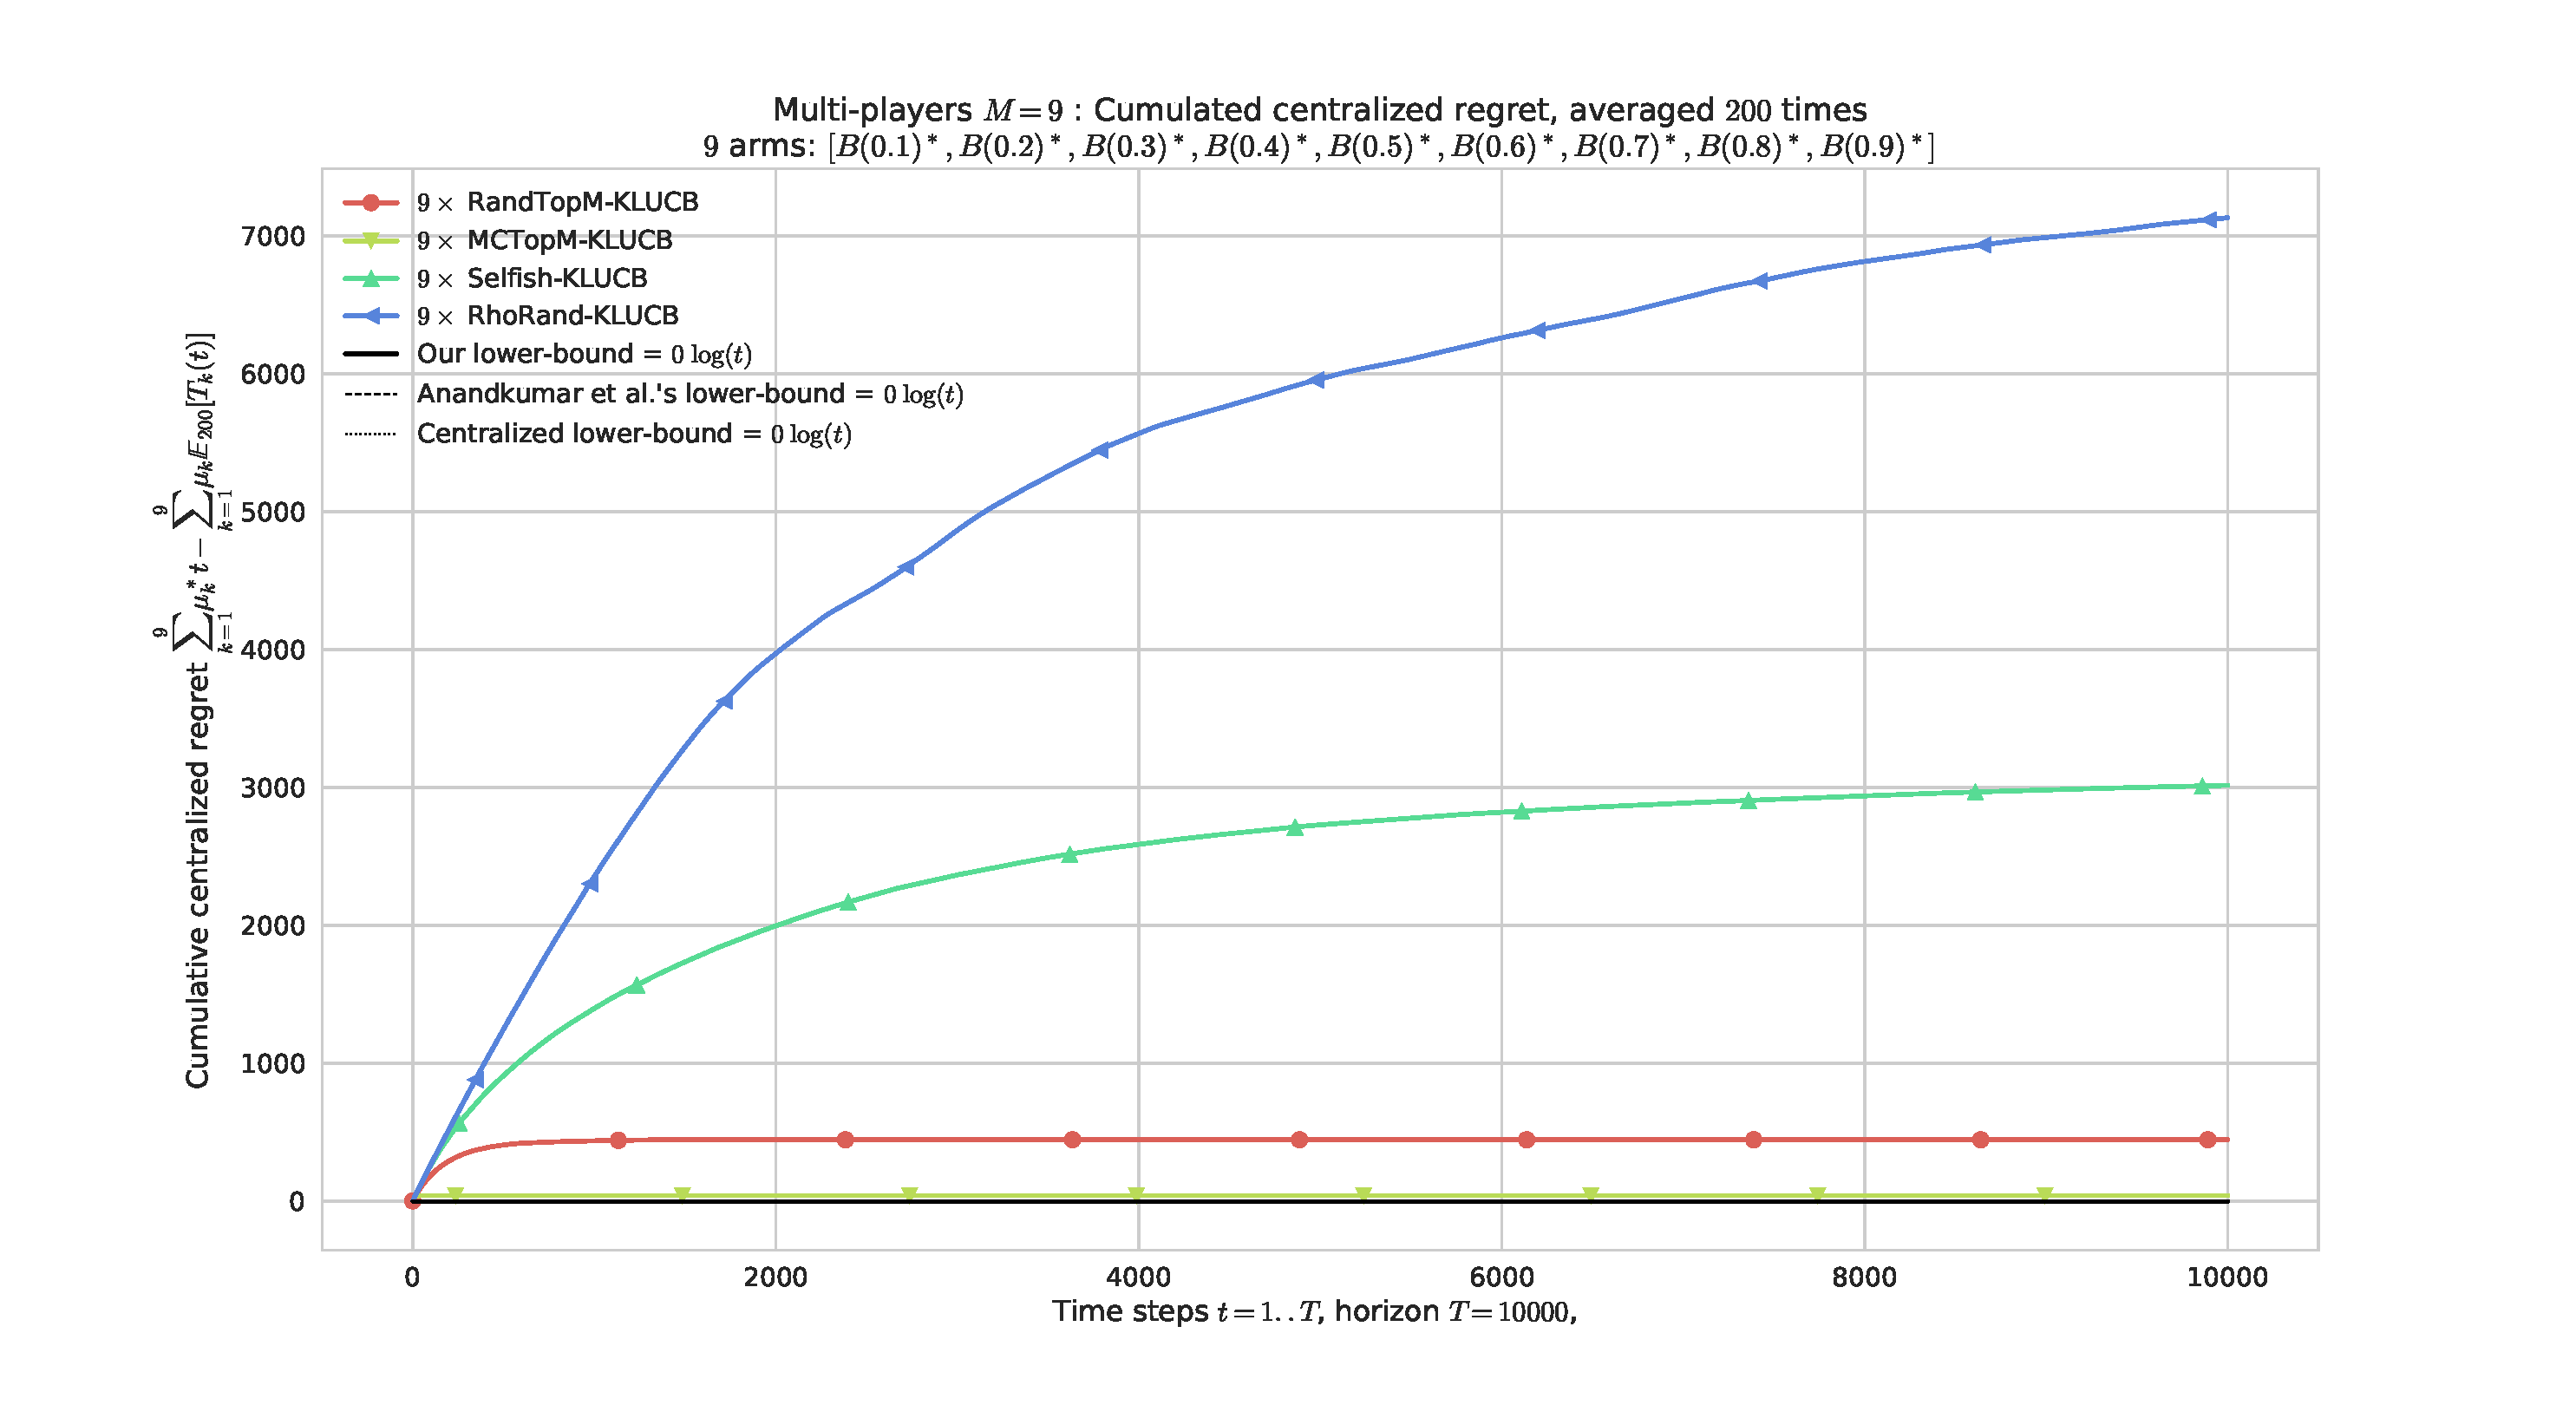
\includegraphics[height=0.75\textheight]{figures/MP__K9_M9_T10000_N200__4_algos/all_RegretCentralized____env1-1_2306423191427933958.pdf}
\caption{\footnotesize{Regret, $M=9$ players, $K=9$ arms, horizon $T=10000$, $200$ repetitions. Only \textcolor{red}{\RandTopM{}} and \textcolor{yellowgreen}{\MCTopM{}} achieve constant regret in this saturated case (proved).}}
\end{figure}

\end{frame}

\begin{frame}[plain]{Illustration of regret of different algorithms}

\begin{figure}[h!]
\centering
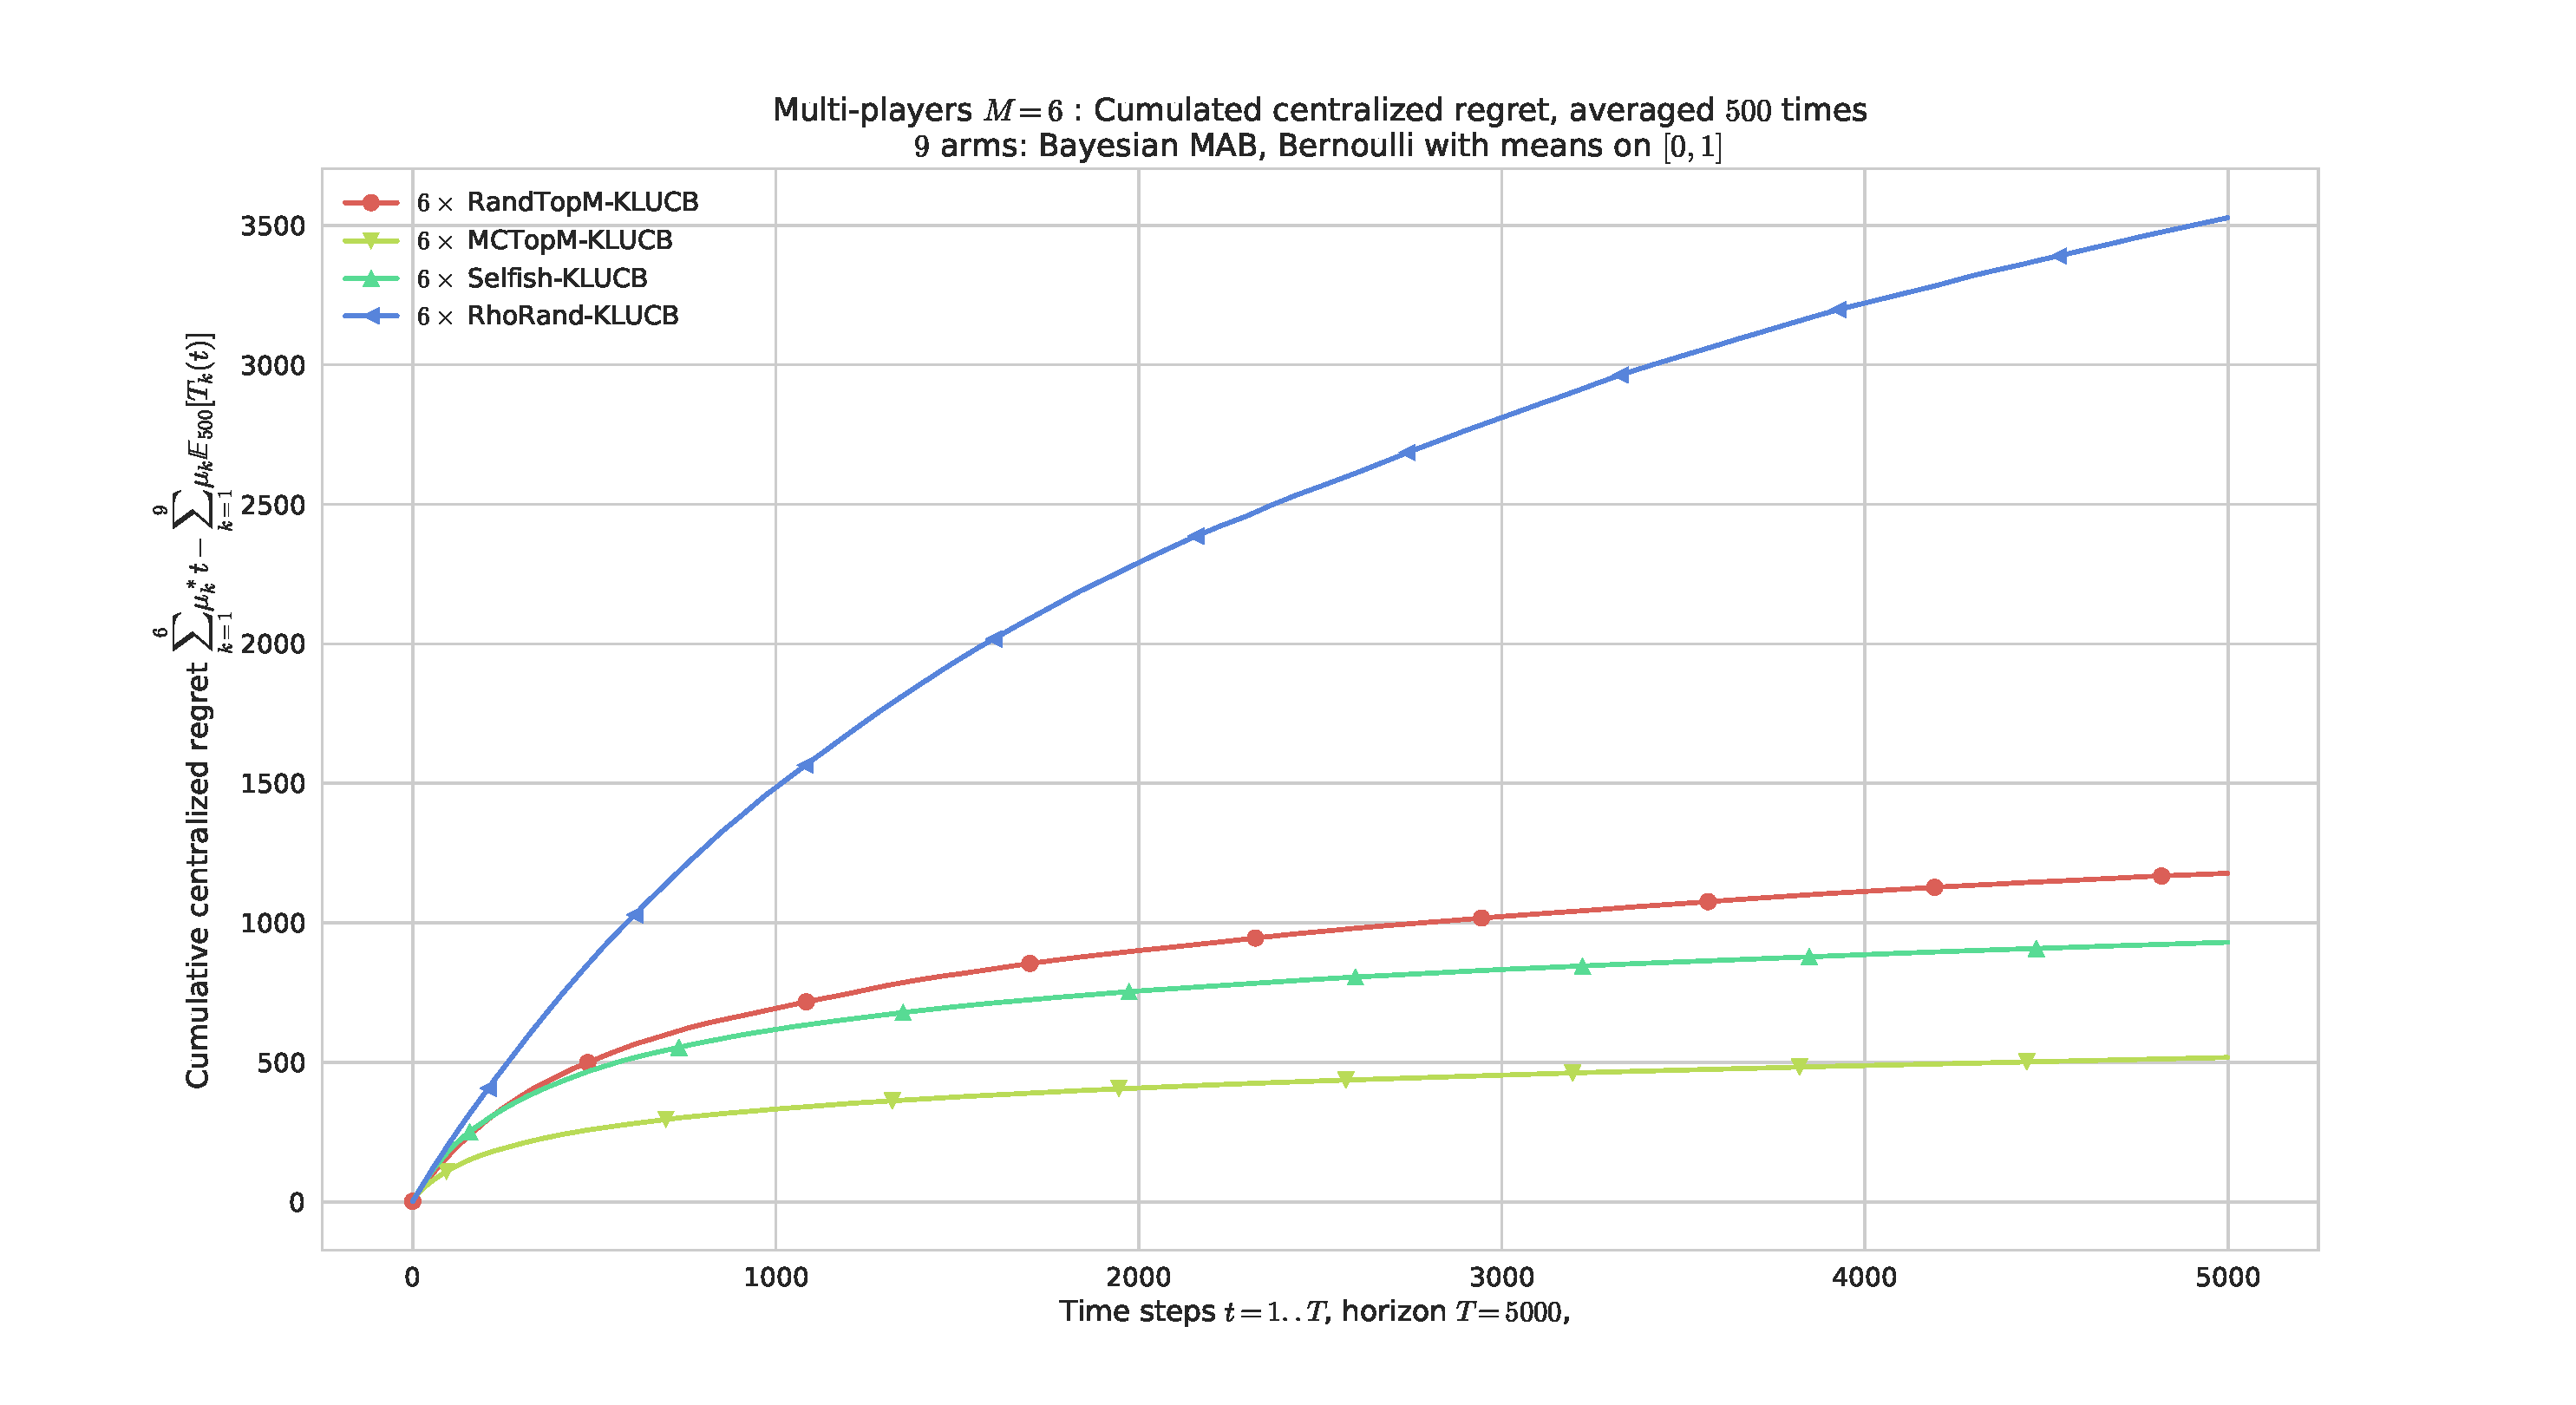
\includegraphics[height=0.75\textheight]{figures/MP__K9_M6_T5000_N500__4_algos/all_RegretCentralized____env1-1_8318947830261751207.pdf}
\caption{\footnotesize{Regret, $M=6$ players, $K=9$ arms, horizon $T=5000$, against $500$ problems $\boldsymbol{\mu}$ uniformly sampled in $[0,1]^K$. Conclusion : \textcolor{blue}{\rhoRand{}} < \textcolor{red}{\RandTopM{}} < \textcolor{bluegreen}{\Selfish{}} < \textcolor{yellowgreen}{\MCTopM{}} in most cases.}}
\end{figure}

\subsection{\hfill{}7.c. Number of collisions\hfill{}}

\end{frame}

\begin{frame}[plain]{Logarithmic number of collisions}

\begin{figure}[h!]
\centering
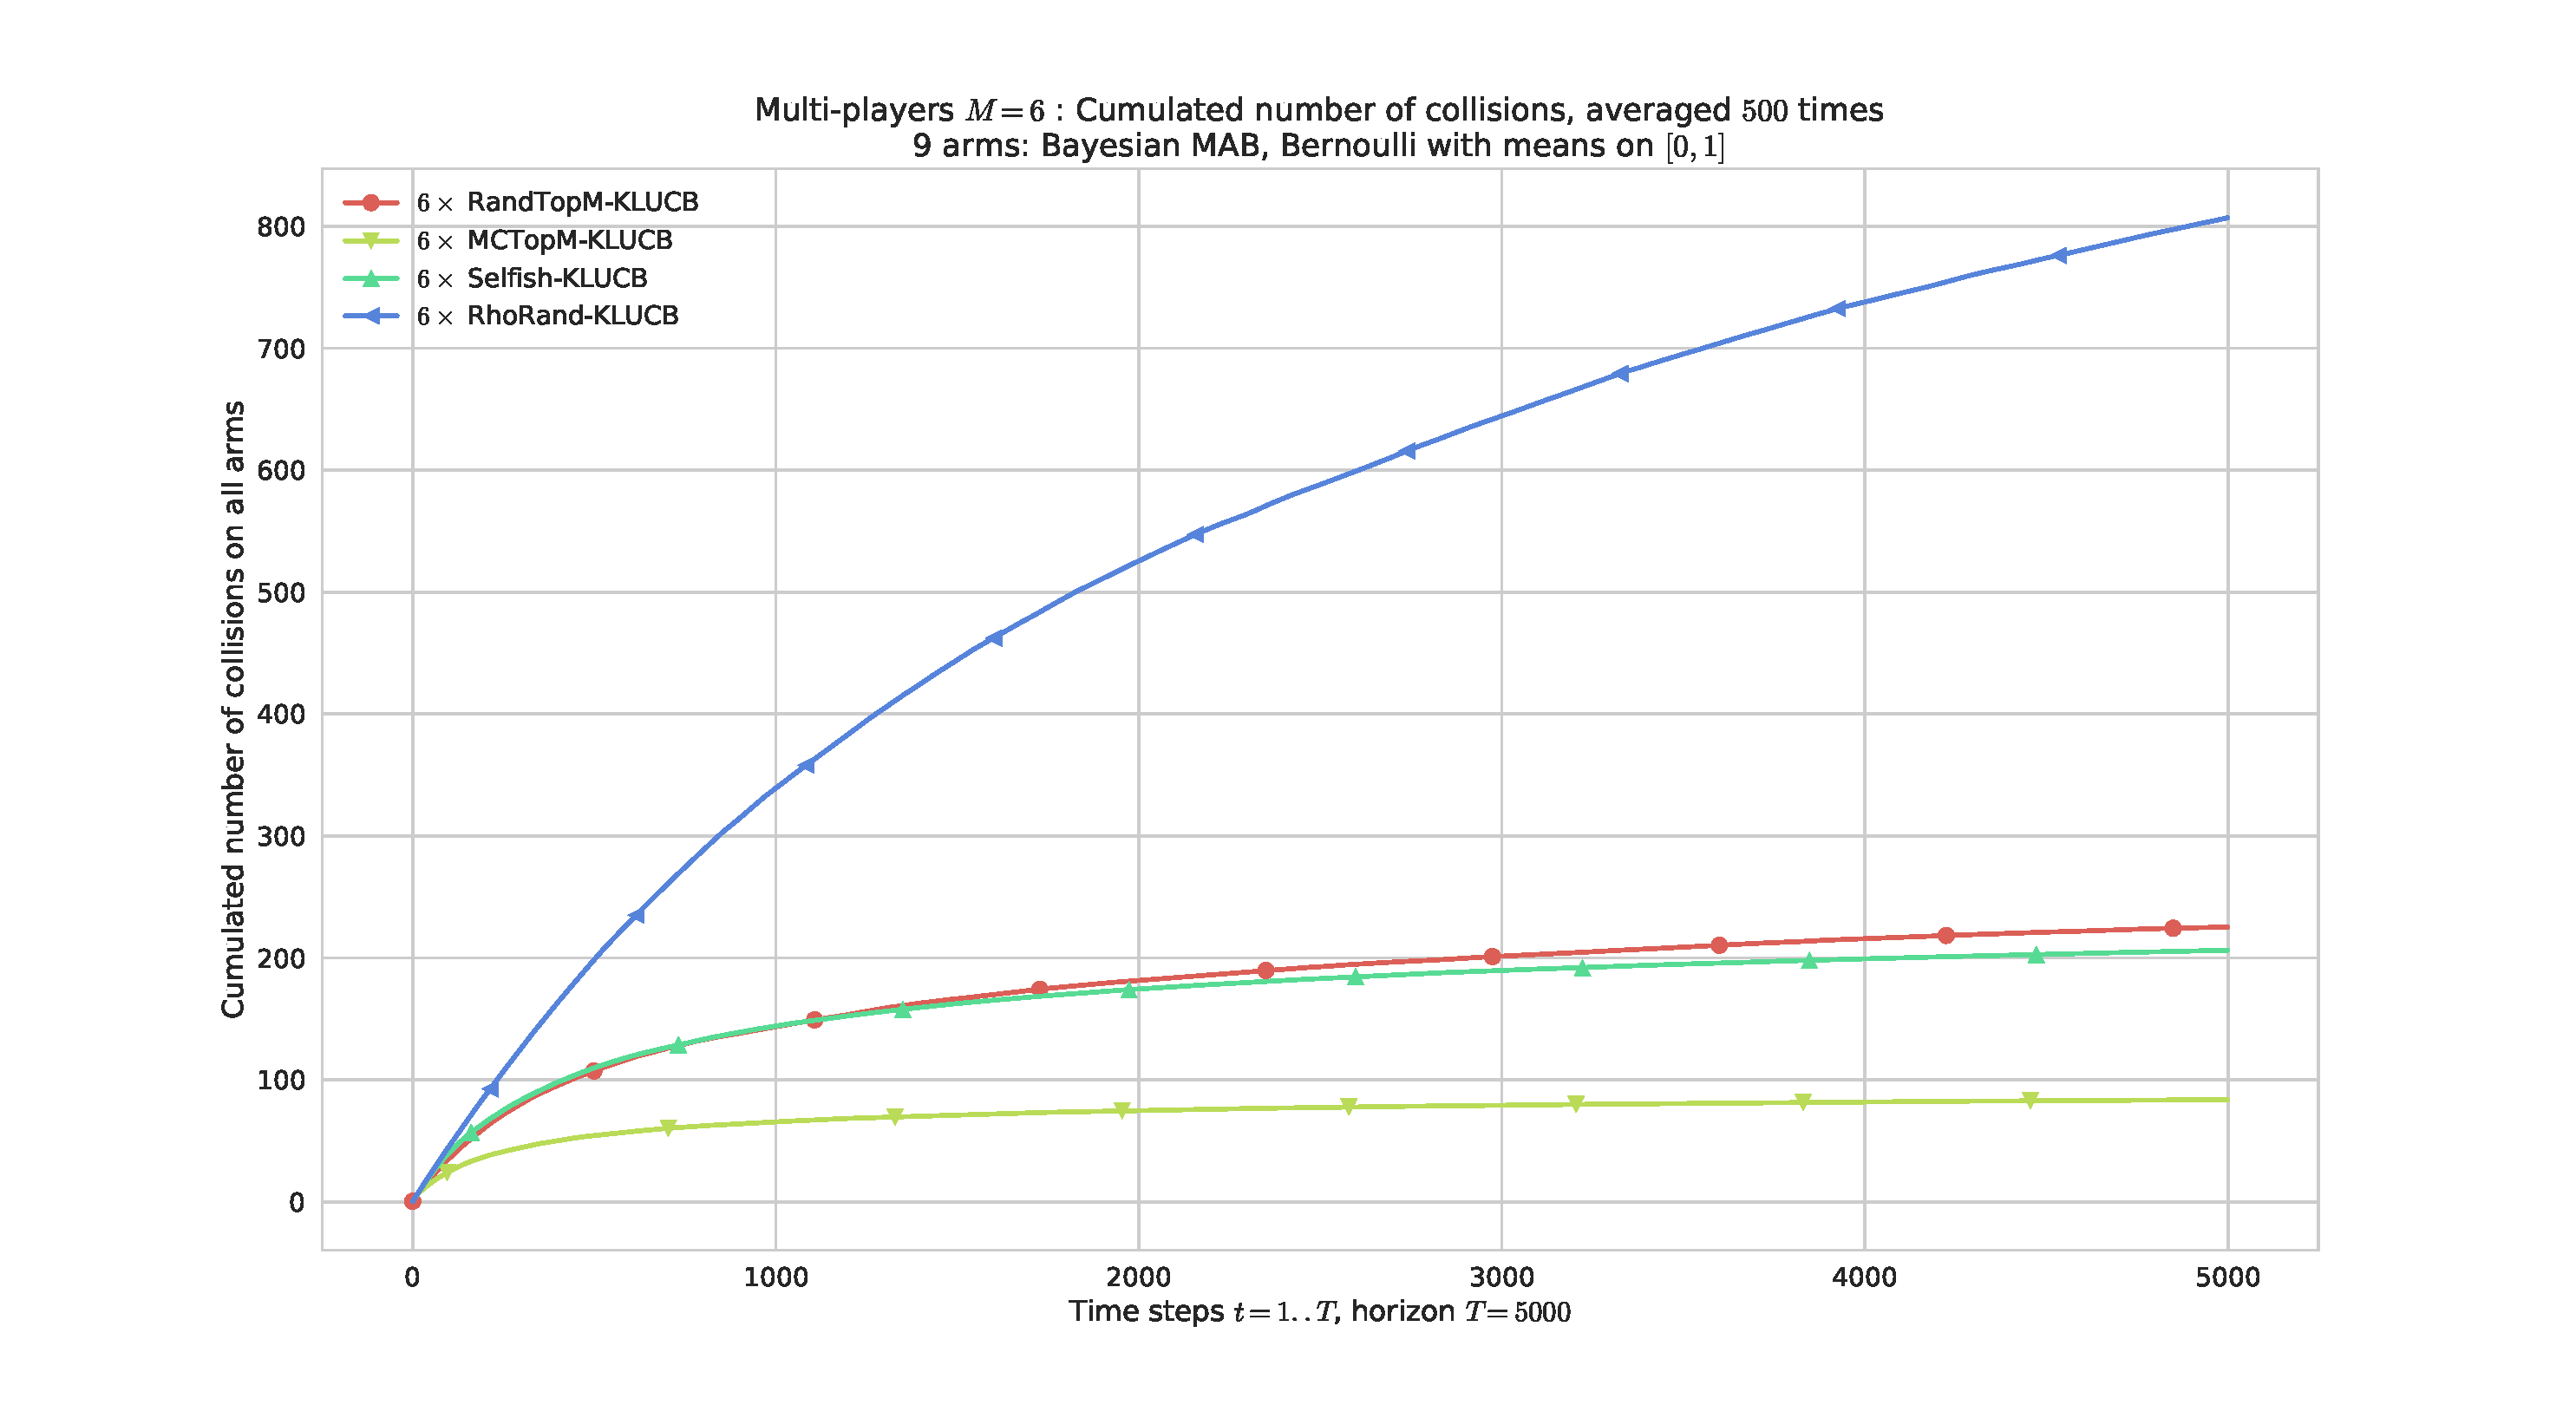
\includegraphics[height=0.75\textheight]{figures/MP__K9_M6_T5000_N500__4_algos/all_CumNbCollisions____env1-1_8318947830261751207.pdf}
\caption{\footnotesize{Cumulated number of collisions. Also \textcolor{blue}{\rhoRand{}} < \textcolor{red}{\RandTopM{}} < \textcolor{bluegreen}{\Selfish{}} < \textcolor{yellowgreen}{\MCTopM{}}.}}
\end{figure}

\subsection{\hfill{}7.d. Number of arm switches\hfill{}}

\end{frame}

\begin{frame}[plain]{Logarithmic number of arm switches}

\begin{figure}[h!]
\centering
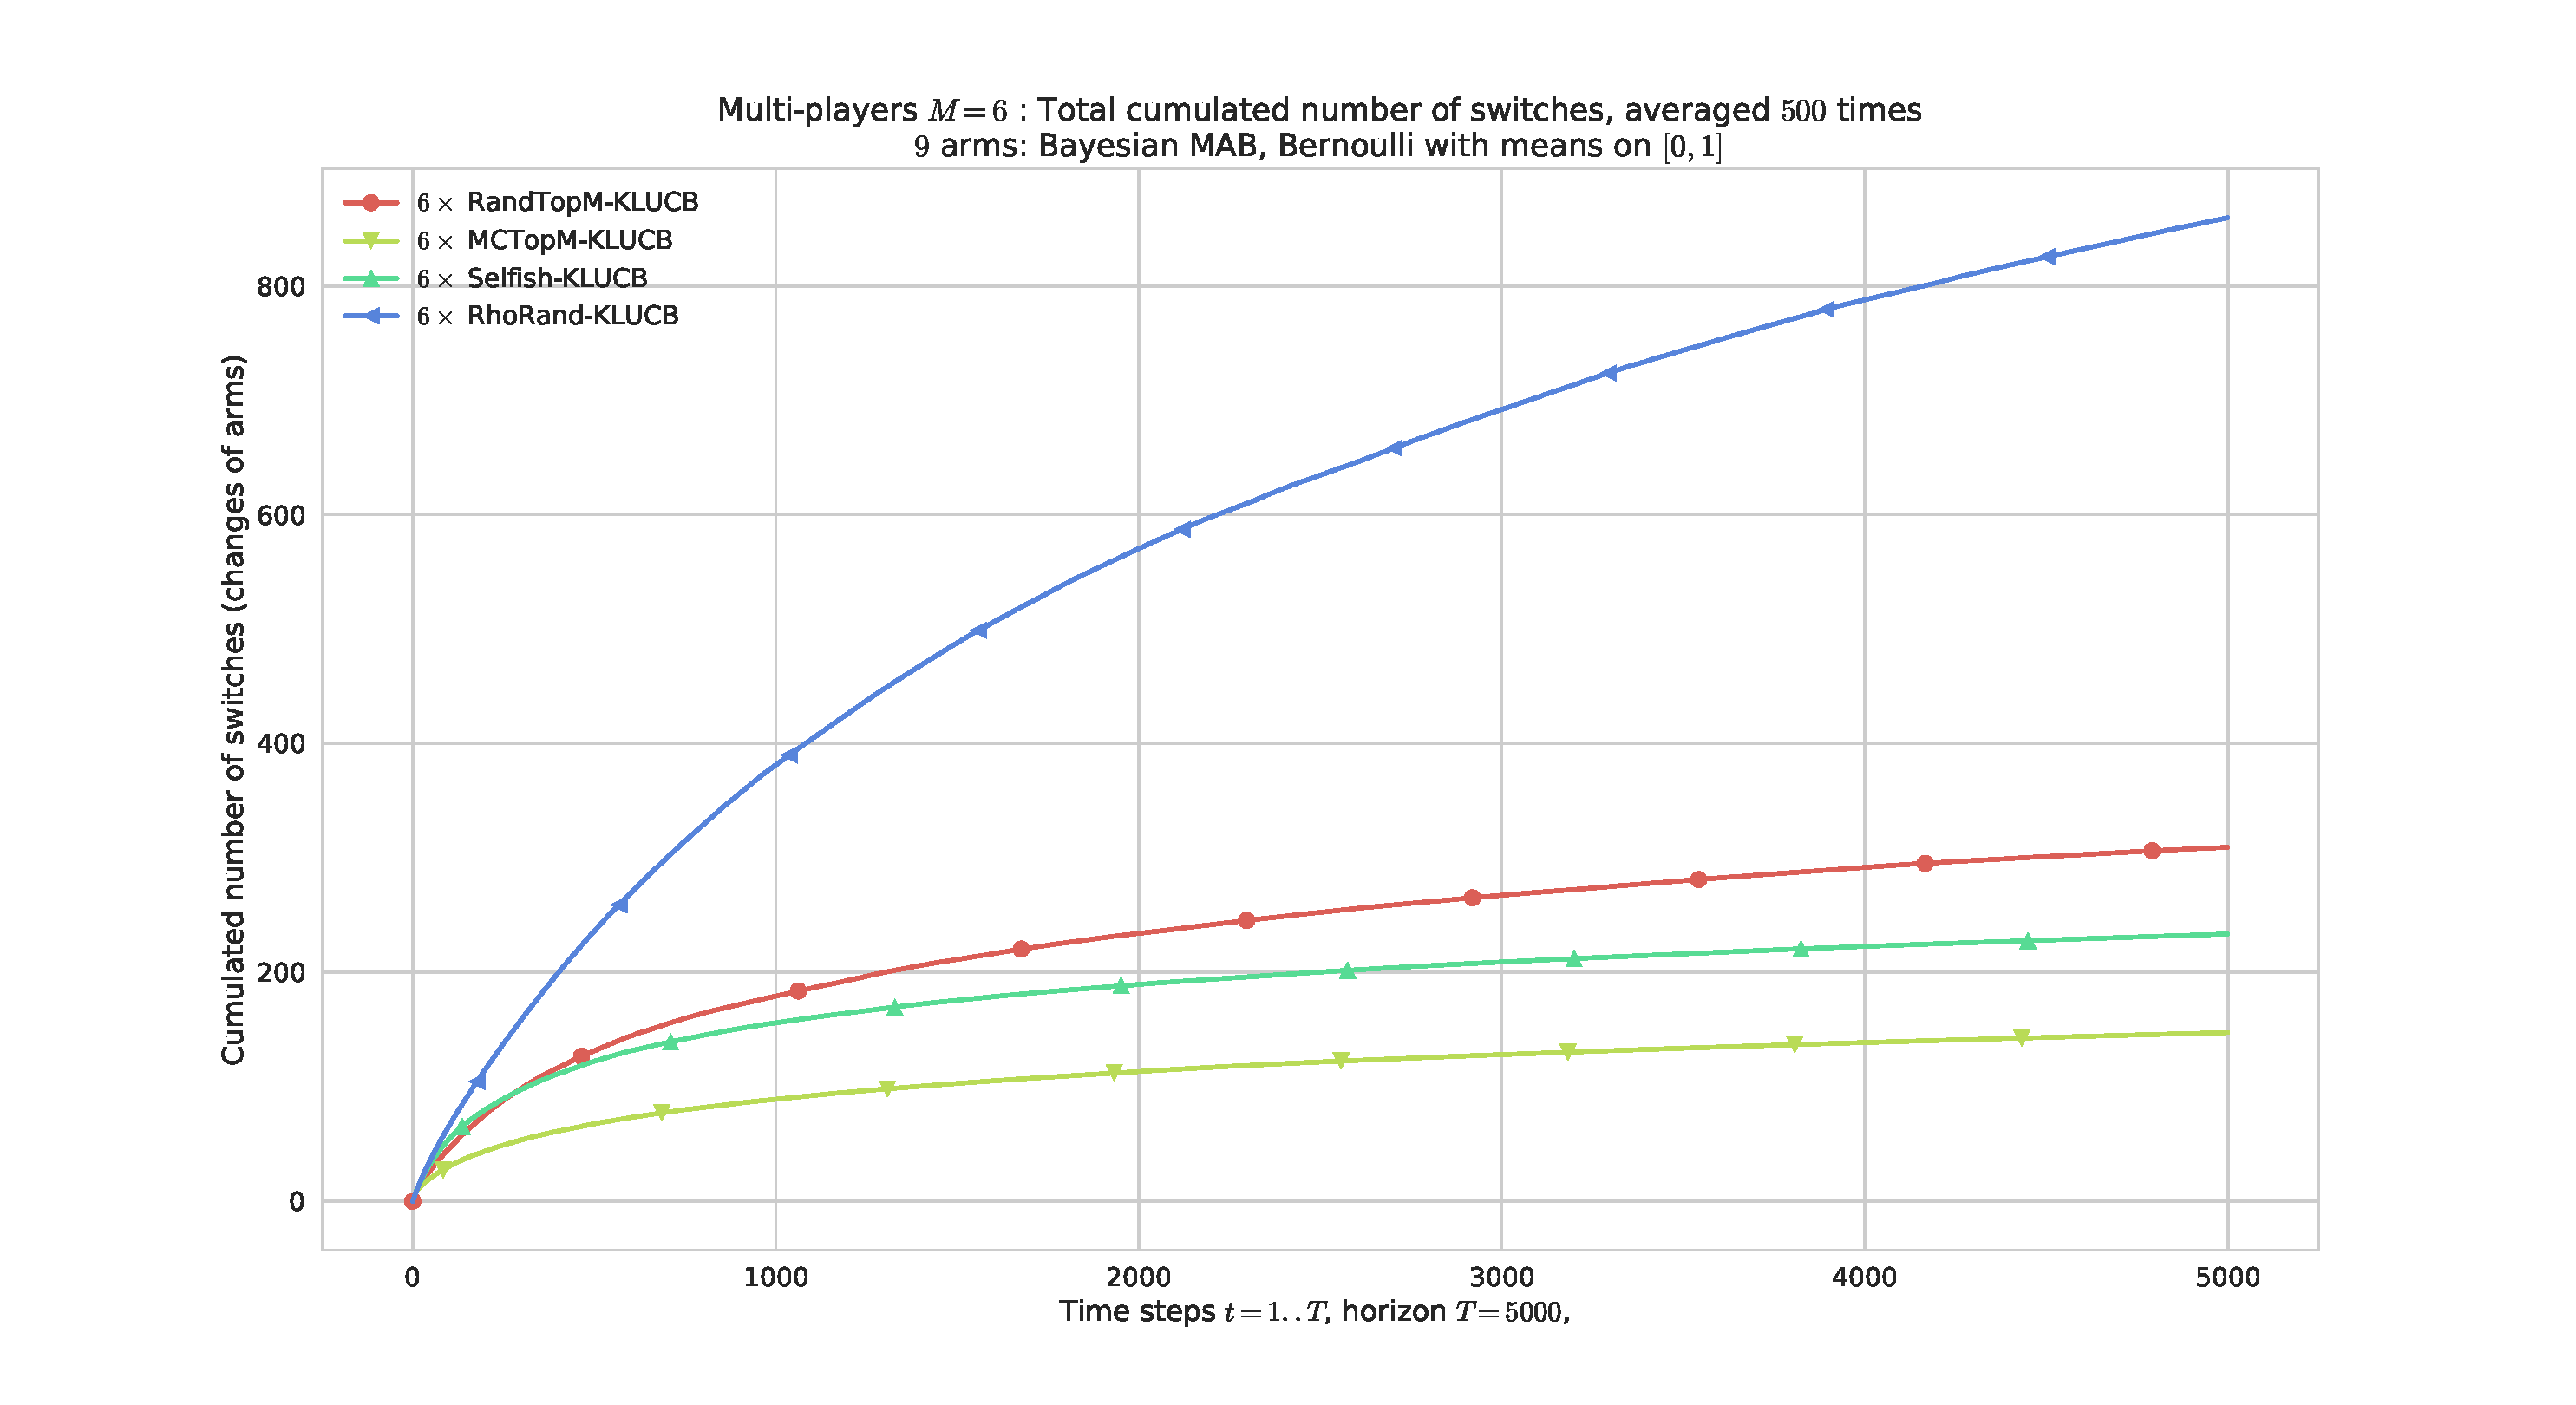
\includegraphics[height=0.75\textheight]{figures/MP__K9_M6_T5000_N500__4_algos/all_CumNbSwitchs____env1-1_8318947830261751207.pdf}
\caption{\footnotesize{Cumulated number of arm switches. Again \textcolor{blue}{\rhoRand{}} < \textcolor{red}{\RandTopM{}} < \textcolor{bluegreen}{\Selfish{}} < \textcolor{yellowgreen}{\MCTopM{}}, but no guarantee for \textcolor{blue}{\rhoRand{}}.}}
\end{figure}

\subsection{\hfill{}7.e. Fairness\hfill{}}

\end{frame}

\begin{frame}[plain]{Fairness}

\begin{figure}[h!]
\centering
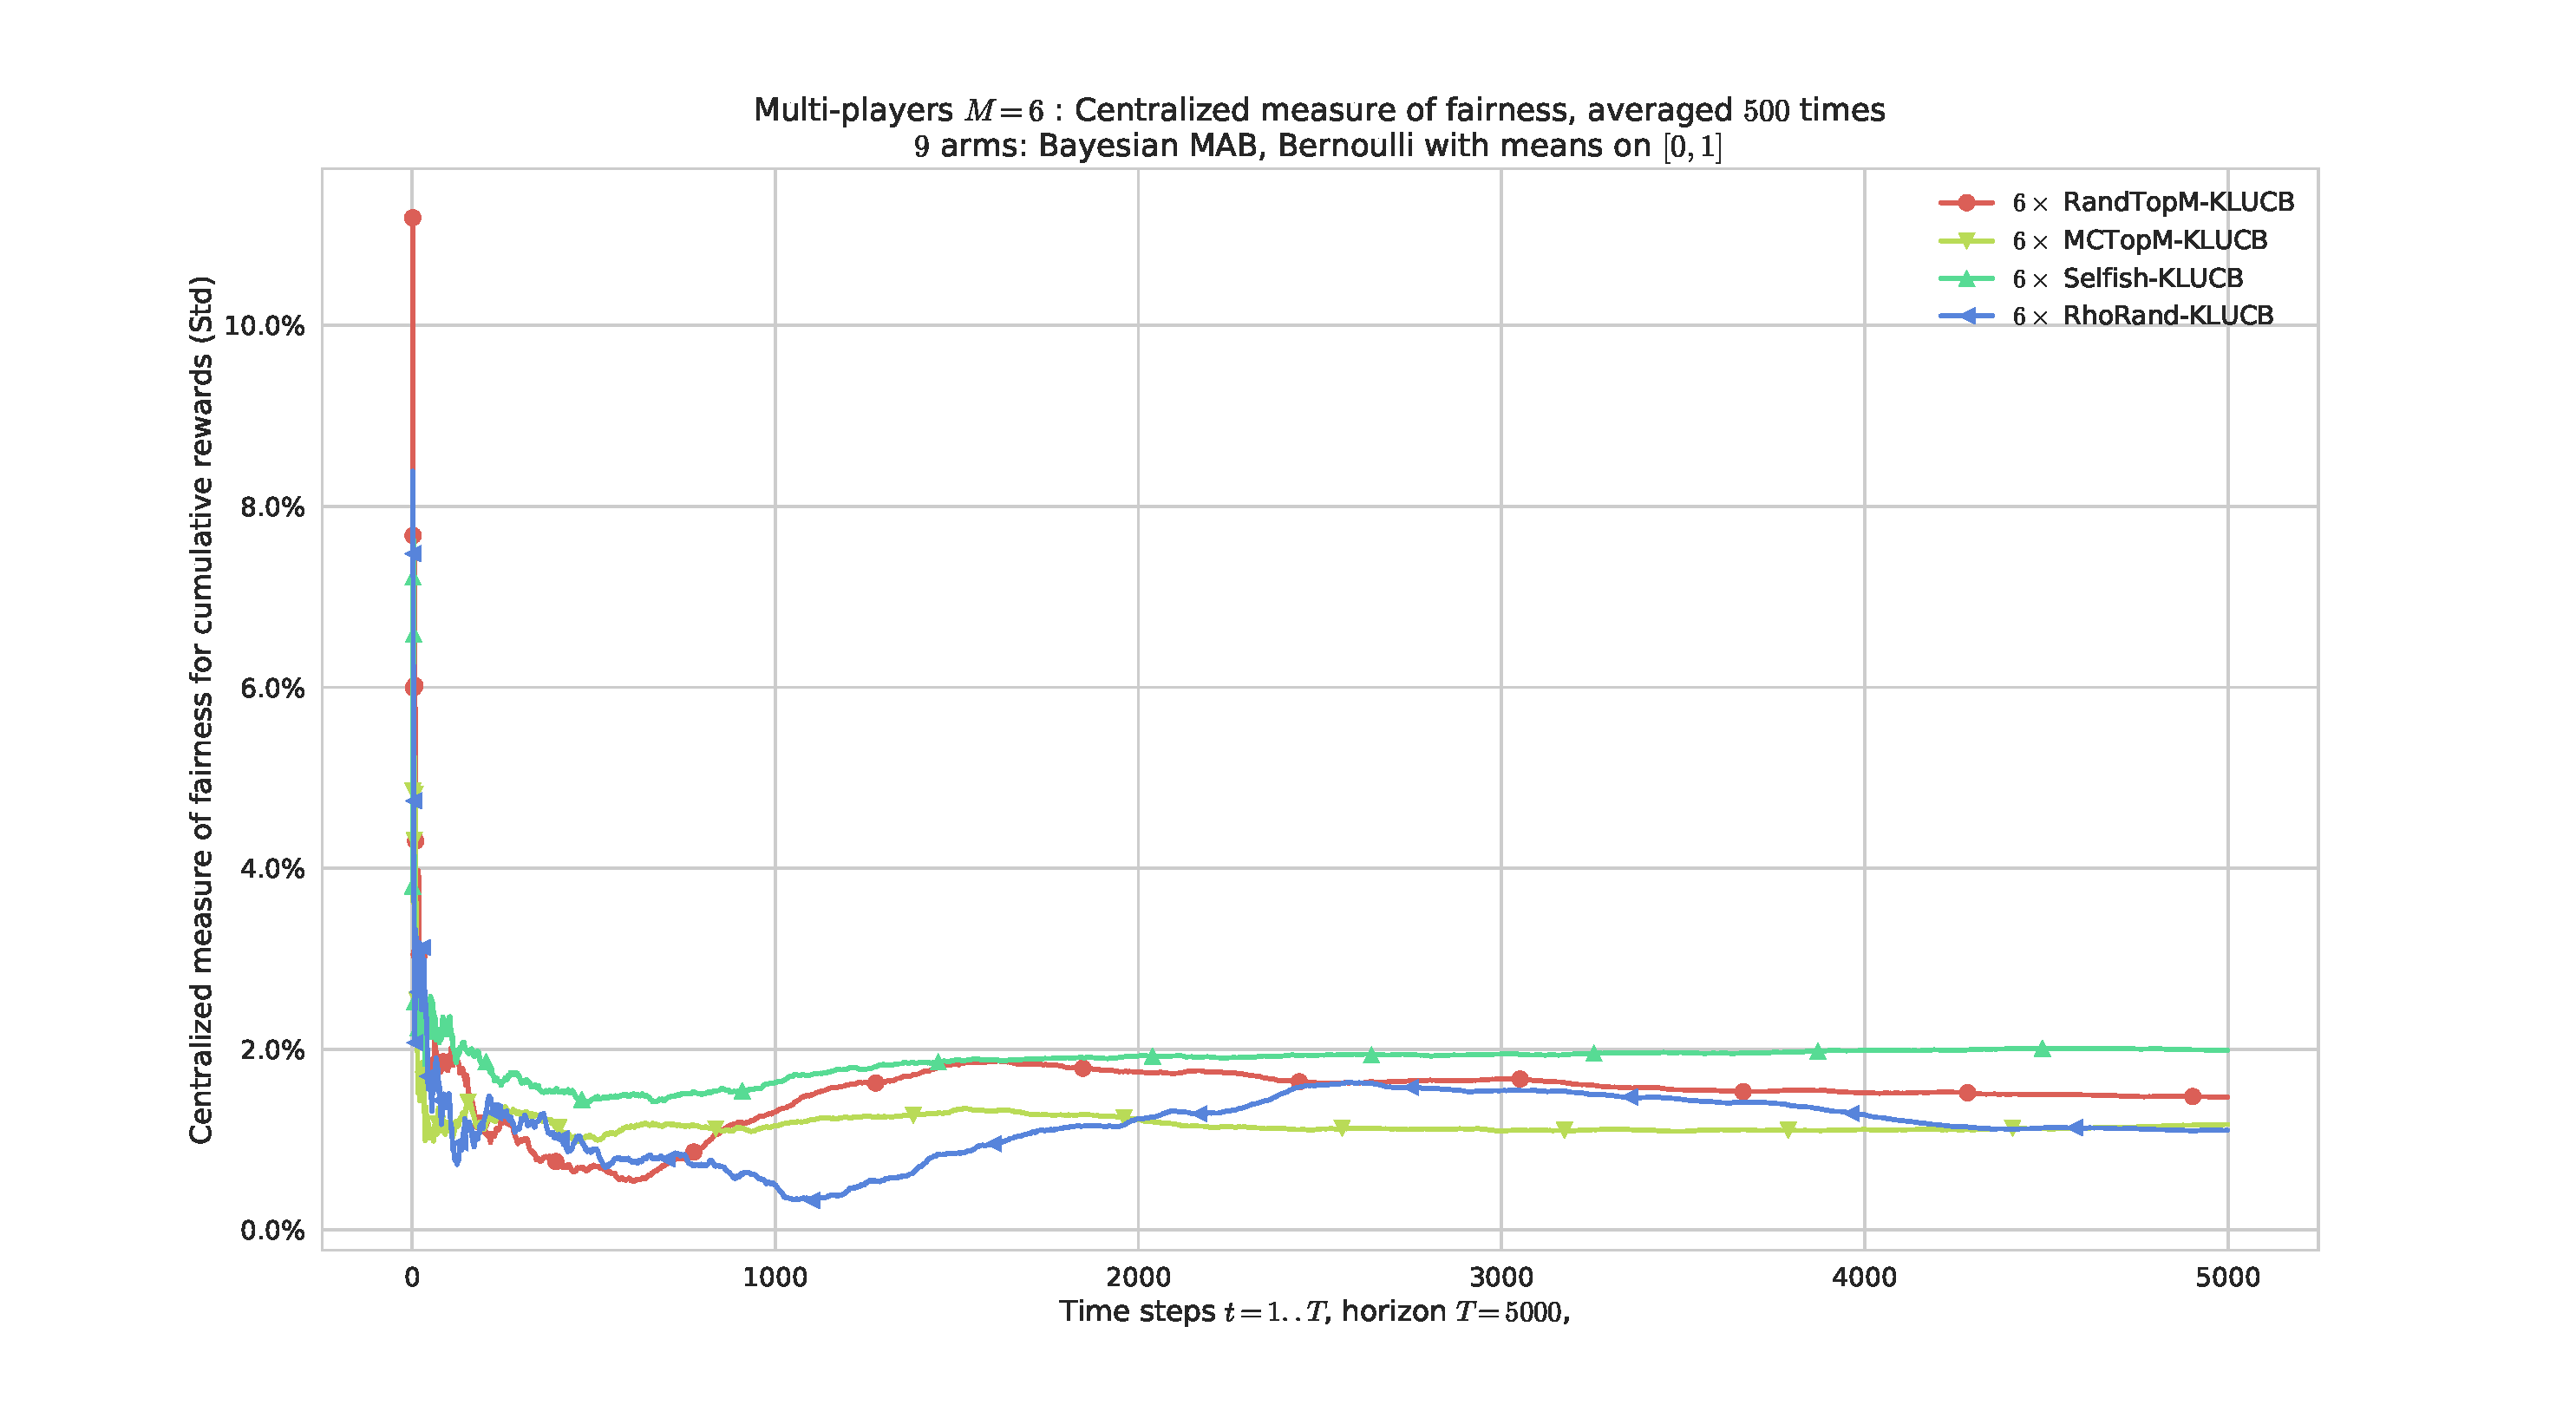
\includegraphics[height=0.75\textheight]{figures/MP__K9_M6_T5000_N500__4_algos/all_FairnessSTD____env1-1_8318947830261751207.pdf}
\caption{\footnotesize{Measure of fairness among player. All $4$ algorithms seem fair \textbf{in average}, but none is fair on a single run. \textbf{It's quite hard to achieve both effiency and single-run fairness!}}}
\end{figure}

\end{frame}



\section{\hfill{}8. An heuristic, \Selfish\hfill{}}

\end{frame}

\begin{frame}{An heuristic, \Selfish}

For the harder feedback model, without sensing.

\begin{enumerate}
\def\labelenumi{\arabic{enumi}.}
\tightlist
\item
  Just an heuristic,\vspace*{15pt}
\item
  Problems with \Selfish,\vspace*{15pt}
\item
  Illustration of failure cases.
\end{enumerate}

\end{frame}



\subsection{\hfill{}8.a. Problems with \Selfish\hfill{}}

\end{frame}

\begin{frame}[allowframebreaks]{The \Selfish{} heuristic}

The \Selfish{} decentralized approach = device don't use sensing, just
learn on the reward (acknowledgement or not, \(r^j(t)\)).

\citationright{Reference: [Bonnefoi \& Besson et al, 2017]}

\begin{block}{Works fine\ldots{}}

\begin{itemize}
\tightlist
\item
  More suited to model IoT networks,
\item
  Use less information, and don't know the value of \(M\): we expect
  \Selfish{} to not have stronger guarantees.
\item
  It works fine in practice!
\end{itemize}

\end{block}

\begin{block}{\emph{But why would it work?}}

\begin{itemize}
\tightlist
\item
  Sensing was \iid{} so using \UCB{} to learn the \(\mu_k\) makes sense,
\item
  But collisions are not \iid,
\item
  Adversarial algorithms are more appropriate here,
\item
  But empirically, \Selfish{} works much better with \UCB{} or \klUCB{}
  than, \eg, \ExpThree\ldots{}
\end{itemize}

\end{block}

\begin{block}{Works fine\ldots{}}

\begin{itemize}
\tightlist
\item
  Except\ldots{} when it fails drastically! \Sadey[1.3]
\item
  In small problems with \(M\) and \(K = 2\) or \(3\), we found small
  probability of failures (\ie, linear regret), and this prevents from
  having a generic upper bound on regret for \Selfish.
\end{itemize}

\end{block}

\end{frame}



\subsection{\hfill{}8.b. Failing cases for \Selfish\hfill{}}

\end{frame}

\begin{frame}[plain]{Illustration of failing cases for
\(\mathrm{Selfish}\)}

\begin{figure}[h!]
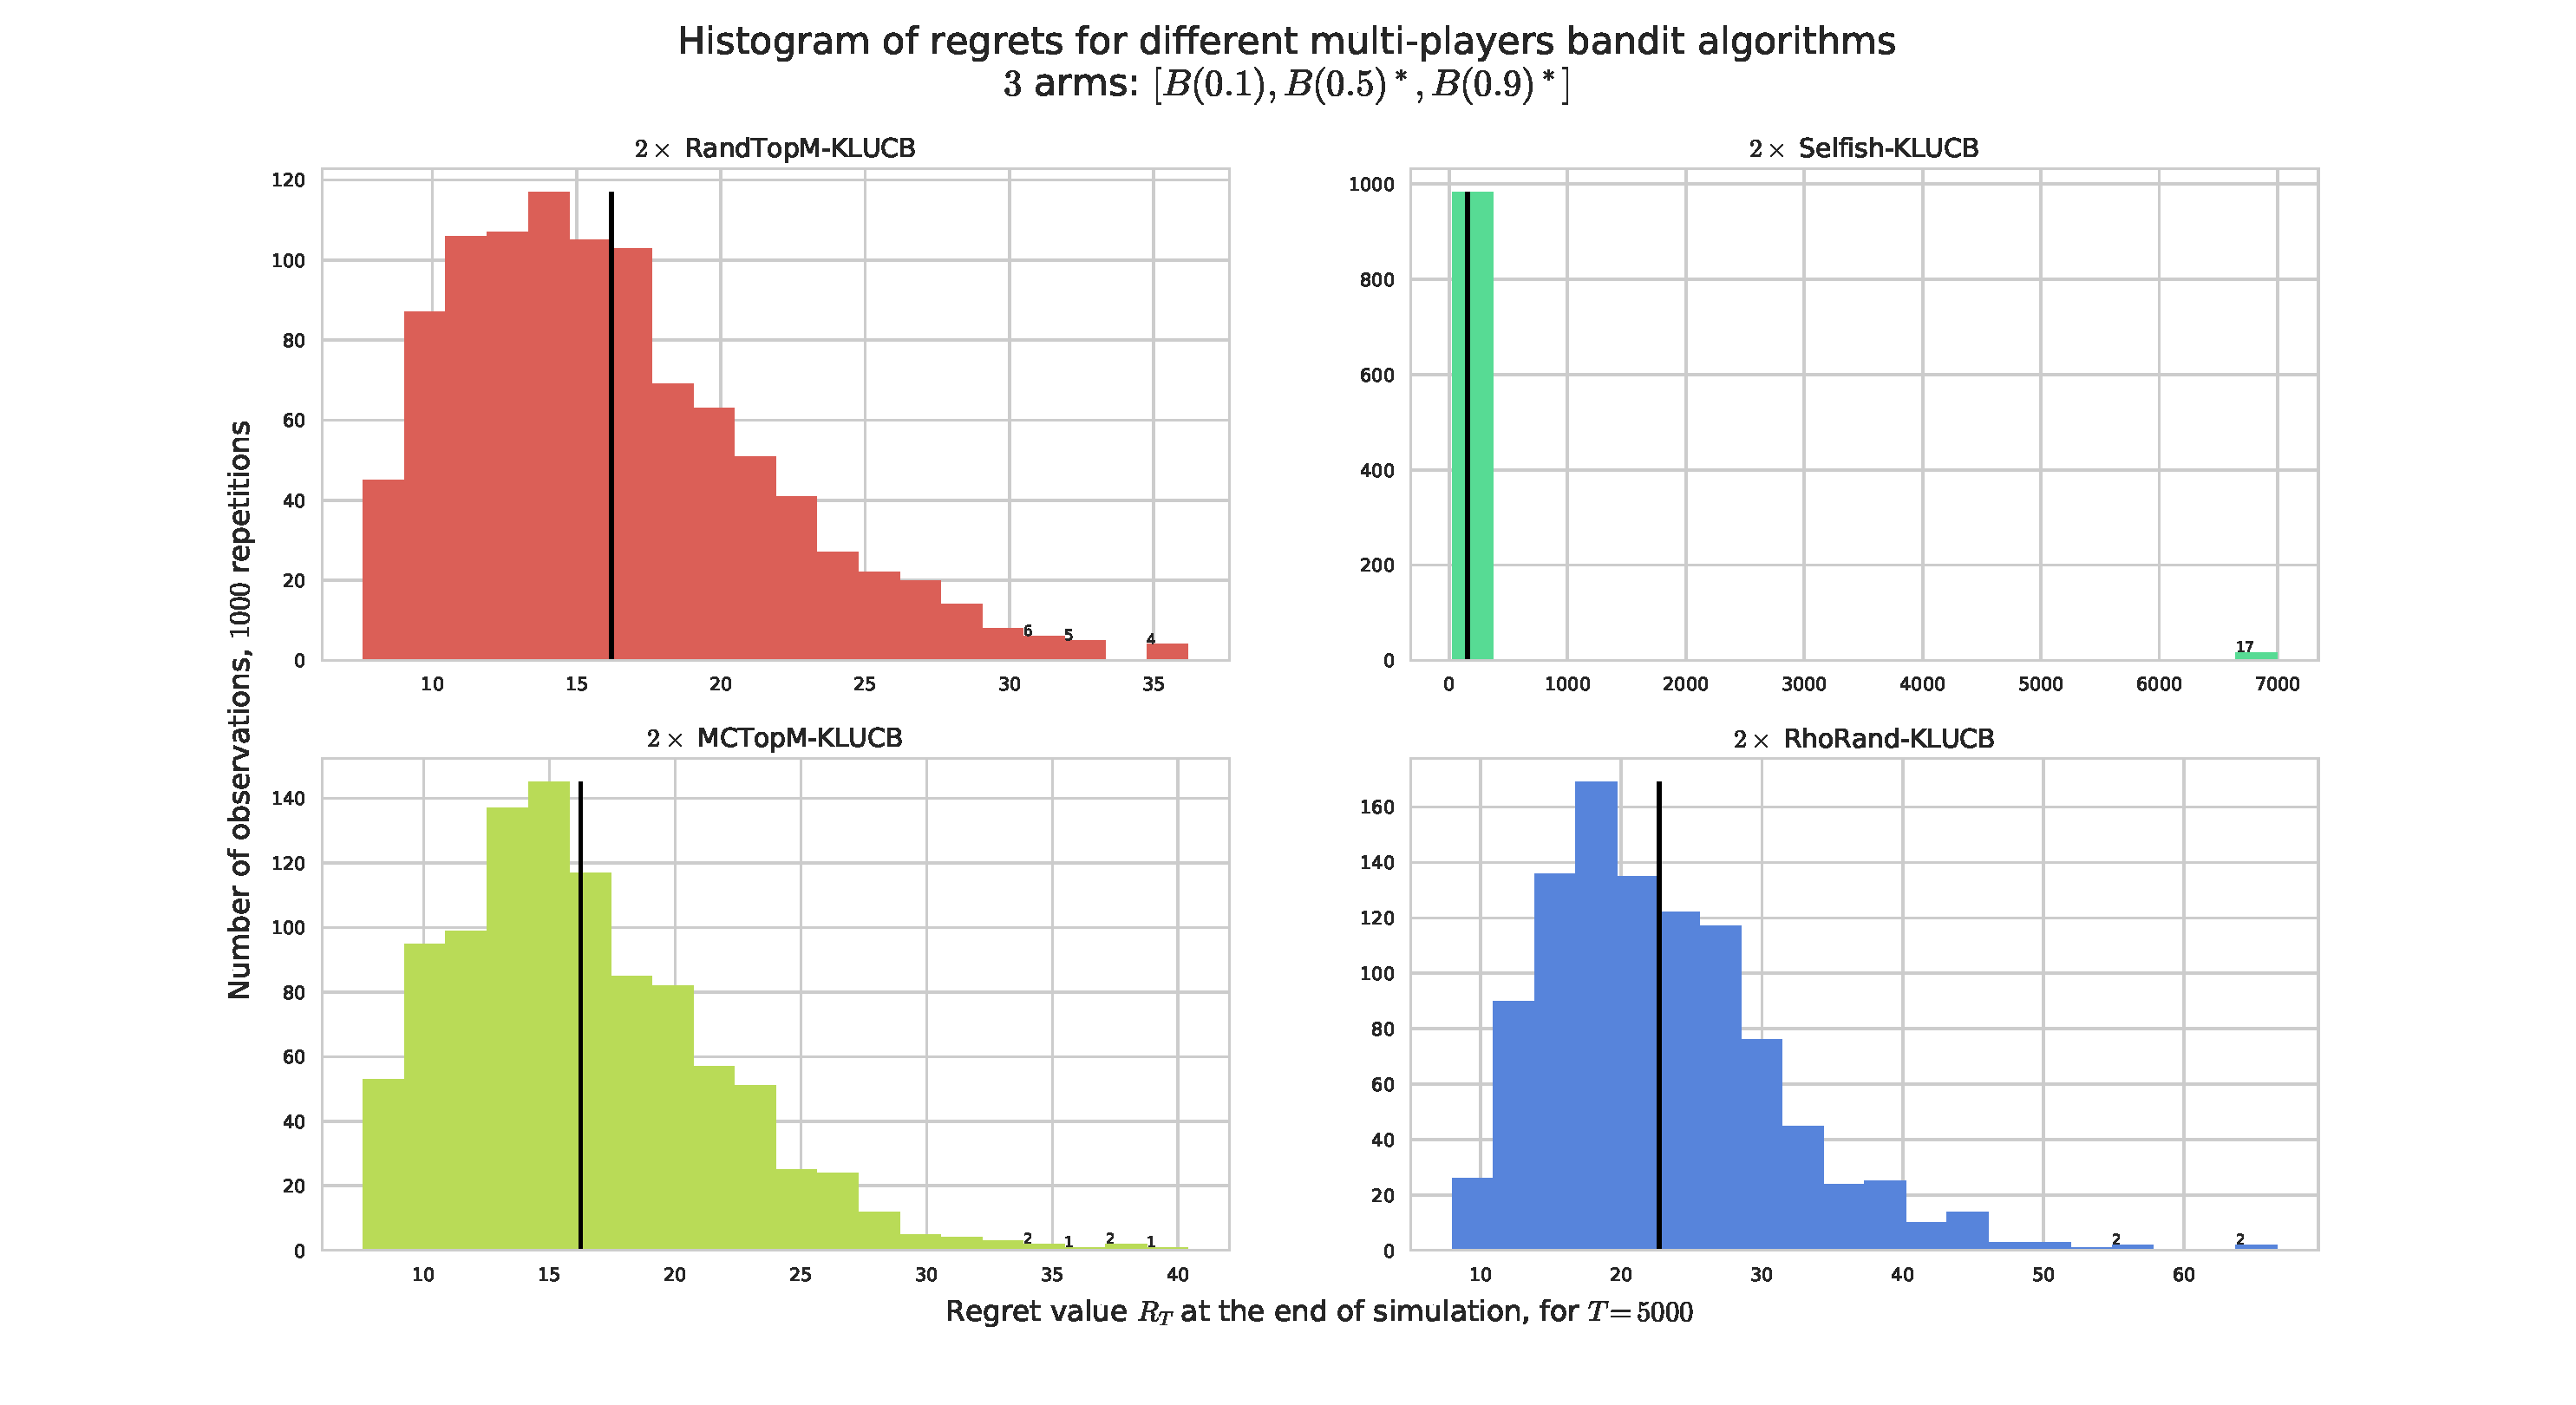
\includegraphics[height=0.70\textheight]{figures/MP__K3_M2_T5000_N1000__4_algos/all_HistogramsRegret____env1-1_5016720151160452442.pdf}
\caption{\footnotesize{Regret for $M=2$, $K=3$, $T=5000$, $1000$ repetitions and $\boldsymbol{\mu} = [0.1, 0.5, 0.9]$. Axis $x$ is for regret (different scale for each), and \textcolor{bluegreen}{\Selfish{}} have a small probability of failure ($17/1000$ cases of $R_T \gg \log T$). The regret for the three other algorithms is very small for this ``easy'' problem.}}
\end{figure}

\end{frame}



\section{\hfill{}9. Conclusion\hfill{}}\subsection{\hfill{}9.a. Sum-up\hfill{}}

\end{frame}

\begin{frame}{Sum-up}

\begin{block}{\emph{Wait, what was the problem ?}}

\begin{itemize}
\tightlist
\item
  MAB algorithms have guarantees for \emph{i.i.d. settings},
\item
  But here the collisions cancel the \iid{} hypothesis\ldots{}
\item
  Not easy to obtain guarantees in this mixed setting \newline
   (\iid{} emissions process, ``game theoretic'' collisions).
\end{itemize}

\pause

\end{block}

\begin{block}{Theoretical results}

\begin{itemize}
\tightlist
\item
  With sensing (``OSA''), we obtained strong results: a lower bound, and
  an order-optimal algorithm,
\item
  But without sensing (``IoT''), it is harder\ldots{} our heuristic
  \Selfish{} usually works but can fail!
\end{itemize}

\end{block}

\end{frame}



\subsection{\hfill{}9.b. Future work\hfill{}}

\end{frame}

\begin{frame}{Other directions of future work}

\begin{block}{Conclude the Multi-Player OSA analysis}

\begin{itemize}
\item
  Remove hypothesis that objects know \(M\),
\item
  Allow arrival/departure of objects,
\item
  Non-stationarity of background traffic etc
\item
  \emph{More realistic emission model}: maybe driven by number of
  packets in a whole day, instead of emission probability.
\end{itemize}

\pause

\end{block}

\begin{block}{Extend to more objects \(M > K\)}

\begin{itemize}
\tightlist
\item
  Extend the theoretical analysis to the large-scale IoT model, first
  with sensing (\eg, models ZigBee networks), then without sensing (\eg,
  LoRaWAN networks).
\end{itemize}

\end{block}

\end{frame}



\subsection{\hfill{}9.c. Thanks!\hfill{}}

\end{frame}

\begin{frame}[allowframebreaks]{Conclusion}

\begin{itemize}
\tightlist
\item
  In a wireless network with an \iid{} background traffic in \(K\)
  channels,
\item
  \(M\) devices can use both sensing and acknowledgement feedback, to
  learn the most free channels and to find orthogonal configurations.
\end{itemize}

\begin{block}{We showed \Smiley[1.2]}

\begin{itemize}
\tightlist
\item
  Decentralized bandit algorithms can solve this problem,
\item
  We have a lower bound for any decentralized algorithm,
\item
  And we proposed an order-optimal algorithm, based on \klUCB{} and an
  improved Musical Chair scheme, \MCTopM
\end{itemize}

\end{block}

\begin{block}{But more work is still needed\ldots{} \Sey[1.2]}

\begin{itemize}
\tightlist
\item
  \textbf{Theoretical guarantees} are still missing for the ``IoT''
  model (without sensing), and can be improved (slightly) for the
  ``OSA'' model (with sensing).
\item
  Maybe study \textbf{other emission models}\ldots{}
\item
  Implement and test this on \textbf{real-world radio devices}
  \hook demo (in progress) for the ICT \(2018\) conference!
\end{itemize}

\end{block}

\begin{block}{\textbf{Thanks!} \Smiley[1.2]}

\begin{center}\begin{Large}
\emph{Any question or idea ?}
\end{Large}\end{center}

\end{block}

\end{frame}

\end{document}
